\documentclass[]{article}
\usepackage{lmodern}
\usepackage{amssymb,amsmath}
\usepackage{ifxetex,ifluatex}
\usepackage{fixltx2e} % provides \textsubscript
\ifnum 0\ifxetex 1\fi\ifluatex 1\fi=0 % if pdftex
  \usepackage[T1]{fontenc}
  \usepackage[utf8]{inputenc}
\else % if luatex or xelatex
  \ifxetex
    \usepackage{mathspec}
    \usepackage{xltxtra,xunicode}
  \else
    \usepackage{fontspec}
  \fi
  \defaultfontfeatures{Mapping=tex-text,Scale=MatchLowercase}
  \newcommand{\euro}{€}
\fi
% use upquote if available, for straight quotes in verbatim environments
\IfFileExists{upquote.sty}{\usepackage{upquote}}{}
% use microtype if available
\IfFileExists{microtype.sty}{%
\usepackage{microtype}
\UseMicrotypeSet[protrusion]{basicmath} % disable protrusion for tt fonts
}{}
\usepackage[margin=1in]{geometry}
\usepackage{color}
\usepackage{fancyvrb}
\newcommand{\VerbBar}{|}
\newcommand{\VERB}{\Verb[commandchars=\\\{\}]}
\DefineVerbatimEnvironment{Highlighting}{Verbatim}{commandchars=\\\{\}}
% Add ',fontsize=\small' for more characters per line
\usepackage{framed}
\definecolor{shadecolor}{RGB}{248,248,248}
\newenvironment{Shaded}{\begin{snugshade}}{\end{snugshade}}
\newcommand{\KeywordTok}[1]{\textcolor[rgb]{0.13,0.29,0.53}{\textbf{{#1}}}}
\newcommand{\DataTypeTok}[1]{\textcolor[rgb]{0.13,0.29,0.53}{{#1}}}
\newcommand{\DecValTok}[1]{\textcolor[rgb]{0.00,0.00,0.81}{{#1}}}
\newcommand{\BaseNTok}[1]{\textcolor[rgb]{0.00,0.00,0.81}{{#1}}}
\newcommand{\FloatTok}[1]{\textcolor[rgb]{0.00,0.00,0.81}{{#1}}}
\newcommand{\CharTok}[1]{\textcolor[rgb]{0.31,0.60,0.02}{{#1}}}
\newcommand{\StringTok}[1]{\textcolor[rgb]{0.31,0.60,0.02}{{#1}}}
\newcommand{\CommentTok}[1]{\textcolor[rgb]{0.56,0.35,0.01}{\textit{{#1}}}}
\newcommand{\OtherTok}[1]{\textcolor[rgb]{0.56,0.35,0.01}{{#1}}}
\newcommand{\AlertTok}[1]{\textcolor[rgb]{0.94,0.16,0.16}{{#1}}}
\newcommand{\FunctionTok}[1]{\textcolor[rgb]{0.00,0.00,0.00}{{#1}}}
\newcommand{\RegionMarkerTok}[1]{{#1}}
\newcommand{\ErrorTok}[1]{\textbf{{#1}}}
\newcommand{\NormalTok}[1]{{#1}}
\ifxetex
  \usepackage[setpagesize=false, % page size defined by xetex
              unicode=false, % unicode breaks when used with xetex
              xetex]{hyperref}
\else
  \usepackage[unicode=true]{hyperref}
\fi
\hypersetup{breaklinks=true,
            bookmarks=true,
            pdfauthor={},
            pdftitle={Predicting Weekly Sales at Walmart Stores},
            colorlinks=true,
            citecolor=blue,
            urlcolor=blue,
            linkcolor=magenta,
            pdfborder={0 0 0}}
\urlstyle{same}  % don't use monospace font for urls
\setlength{\parindent}{0pt}
\setlength{\parskip}{6pt plus 2pt minus 1pt}
\setlength{\emergencystretch}{3em}  % prevent overfull lines
\setcounter{secnumdepth}{5}

%%% Use protect on footnotes to avoid problems with footnotes in titles
\let\rmarkdownfootnote\footnote%
\def\footnote{\protect\rmarkdownfootnote}

%%% Change title format to be more compact
\usepackage{titling}

% Create subtitle command for use in maketitle
\newcommand{\subtitle}[1]{
  \posttitle{
    \begin{center}\large#1\end{center}
    }
}

\setlength{\droptitle}{-2em}
  \title{Predicting Weekly Sales at Walmart Stores}
  \pretitle{\vspace{\droptitle}\centering\huge}
  \posttitle{\par}
  \author{}
  \preauthor{}\postauthor{}
  \predate{\centering\large\emph}
  \postdate{\par}
  \date{August 31, 2015}



\begin{document}

\maketitle


{
\hypersetup{linkcolor=black}
\setcounter{tocdepth}{3}
\tableofcontents
}
\pagebreak

\section{1. Executive Summary}\label{executive-summary}

Retail stores need to be able to predict sales forecasts for the future
and study the effect how strategic offers affect sales, especially
during holiday season. Since the number of days in holidays are limited,
it becomes more challenging to be able to accurately predict how
different aspects affect sales.

This report will focus on a Walmart Data set that has Department-wise
Weekly Sales of 45 Walmart stores. It will attempt to create a
predictive model and also discuss the extent to which different factors
affect the sales.

\pagebreak

\section{Introduction}\label{introduction}

\subsection{About the Solution
Environment}\label{about-the-solution-environment}

The authors implemented this solution in R. We have used R Markdown
Report to create this document. First we explore and prepare the data
set before carrying out formal statistical inferences on the data set.
We wrap the report by building a model to predict Weekly sales of the
departments belonging to the 45 stores in this data set.

\subsection{About the Data}\label{about-the-data}

The data set under consideration is taken from a recruitment competition
Walmart ran on Kaggle between February-May 2014. Each store has multiple
departments and the end requirement is to be able to predict the sales
for individual departments of each store.

The training data set has more than 400K records. The testing data set
has over 100K records.

\subsubsection{The Challenge}\label{the-challenge}

The challenge is to be able to predict how different holiday price
markdowns affect the various departments in the store, to model extent
of impact of these markdowns.

\subsection{2.3 Getting the Data}\label{getting-the-data}

The data was download from Kaggle.

URL to the Kaggle Competition Site:
\url{https://www.kaggle.com/c/walmart-recruiting-store-sales-forecasting}

The files available are the following:

\subsubsection{The Data Files}\label{the-data-files}

Here we discuss the various CSV Files that are given by Walmart.

\paragraph{2.3.1.1 stores.csv}\label{stores.csv}

Contains size and type of 45 stores (45 records).

\paragraph{2.3.1.2 train.csv}\label{train.csv}

Weekly sales data set from February 05, 2010 to November 11, 2012. It
contains the following fields:

\begin{itemize}
\itemsep1pt\parskip0pt\parsep0pt
\item
  Store: store number
\item
  Dept: the department number
\item
  Date: week date
\item
  Weekly\_Sales: sales for the given department in the given store
\item
  IsHoliday: whether the week is a special holiday week
\end{itemize}

\paragraph{2.3.1.3 test.csv}\label{test.csv}

The data set with similar fields as train.csv, except without
Weekly\_Sales. This will be used to test the model with unseen data and
can be evaluated by uploading the data set to Kaggle.

\paragraph{2.3.1.4 features.csv}\label{features.csv}

This data file contains additional relevant information relating to the
physical and business environment around the store. The fields are as
follows:

\begin{itemize}
\itemsep1pt\parskip0pt\parsep0pt
\item
  Store: store number
\item
  Date: the week date
\item
  Temperature: the average temperature in the region
\item
  Fuel\_Price: cost of fuel in the region
\item
  MarkDown1-5: data related to the markdowns that Walmart is running.
  Markdown data is only available after November 2011 and is not
  available for all stores all the time. Any missing value is marked
  with an NA.
\item
  CPI - the Consumer Price Index
\item
  Unemployment - the unemployment rate
\item
  IsHoliday - whether the week is a special holiday week
\end{itemize}

The four holidays fall in the following weeks in the data set:

\begin{itemize}
\itemsep1pt\parskip0pt\parsep0pt
\item
  Super Bowl: 12-Feb-10, 11-Feb-11, 10-Feb-12, 8-Feb-13
\item
  Labor Day: 10-Sep-10, 9-Sep-11, 7-Sep-12, 6-Sep-13
\item
  Thanksgiving: 26-Nov-10, 25-Nov-11, 23-Nov-12, 29-Nov-13
\item
  Christmas: 31-Dec-10, 30-Dec-11, 28-Dec-12, 27-Dec-13
\end{itemize}

\subsubsection{2.3.2 Ingesting the Data}\label{ingesting-the-data}

\begin{Shaded}
\begin{Highlighting}[]
\NormalTok{## Ingesting the data from the Data folder: Training Dataset}
\NormalTok{train <-}\StringTok{ }\KeywordTok{read.csv}\NormalTok{(}\StringTok{"Data/train.csv"}\NormalTok{)}
\end{Highlighting}
\end{Shaded}

\begin{Shaded}
\begin{Highlighting}[]
\NormalTok{## Ingesting the data from the Data folder: Stores Dataset}
\NormalTok{stores <-}\StringTok{ }\KeywordTok{read.csv}\NormalTok{(}\StringTok{"Data/stores.csv"}\NormalTok{)}
\end{Highlighting}
\end{Shaded}

\begin{Shaded}
\begin{Highlighting}[]
\NormalTok{## Ingesting the data from the Data folder: features Dataset}
\NormalTok{features <-}\StringTok{ }\KeywordTok{read.csv}\NormalTok{(}\StringTok{"Data/features.csv"}\NormalTok{)}
\end{Highlighting}
\end{Shaded}

\begin{Shaded}
\begin{Highlighting}[]
\NormalTok{## Ingesting the data from the Data folder: testing Dataset}
\NormalTok{test <-}\StringTok{ }\KeywordTok{read.csv}\NormalTok{(}\StringTok{"Data/test.csv"}\NormalTok{)}
\end{Highlighting}
\end{Shaded}

\subsection{2.4 R Libraries Used}\label{r-libraries-used}

The following libraries are used in this report:

\begin{Shaded}
\begin{Highlighting}[]
\CommentTok{# Grammar of Graphics Plotting Library}
\KeywordTok{library}\NormalTok{(ggplot2)}
\CommentTok{# To use 'melt'}
\KeywordTok{library}\NormalTok{(reshape2)}
\CommentTok{# to enable commas in graphs}
\KeywordTok{library}\NormalTok{(scales)}
\CommentTok{# to get the month number from date variable}
\KeywordTok{library}\NormalTok{(lubridate)}
\CommentTok{# to calculate Kurtosis}
\KeywordTok{library}\NormalTok{(e1071)}
\NormalTok{## to be able to plot in grids}
\KeywordTok{library}\NormalTok{(grid)}
\NormalTok{## to be able to plot in grids}
\KeywordTok{library}\NormalTok{(gridExtra)}
\end{Highlighting}
\end{Shaded}

\pagebreak

\section{3. Stage 1: Data Exploration and
Preparation}\label{stage-1-data-exploration-and-preparation}

\subsection{3.1 Summary Statististics}\label{summary-statististics}

\subsubsection{3.1.1 The Training Dataset
(train)}\label{the-training-dataset-train}

This is the structure of the dataset

\begin{verbatim}
## 'data.frame':    421570 obs. of  5 variables:
##  $ Store       : int  1 1 1 1 1 1 1 1 1 1 ...
##  $ Dept        : int  1 1 1 1 1 1 1 1 1 1 ...
##  $ Date        : Factor w/ 143 levels "2010-02-05","2010-02-12",..: 1 2 3 4 5 6 7 8 9 10 ...
##  $ Weekly_Sales: num  24924 46039 41596 19404 21828 ...
##  $ IsHoliday   : logi  FALSE TRUE FALSE FALSE FALSE FALSE ...
\end{verbatim}

Date is ingested as factor (as opposed to being ingested as date type).
There are 143 dates in total.

\begin{verbatim}
##      Store           Dept            Date             Weekly_Sales   
##  Min.   : 1.0   Min.   : 1.00   Min.   :2010-02-05   Min.   : -4989  
##  1st Qu.:11.0   1st Qu.:18.00   1st Qu.:2010-10-08   1st Qu.:  2080  
##  Median :22.0   Median :37.00   Median :2011-06-17   Median :  7612  
##  Mean   :22.2   Mean   :44.26   Mean   :2011-06-18   Mean   : 15981  
##  3rd Qu.:33.0   3rd Qu.:74.00   3rd Qu.:2012-02-24   3rd Qu.: 20206  
##  Max.   :45.0   Max.   :99.00   Max.   :2012-10-26   Max.   :693099  
##  IsHoliday      
##  Mode :logical  
##  FALSE:391909   
##  TRUE :29661    
##  NA's :0        
##                 
## 
\end{verbatim}

 There is no missing data in the data set.

As discussed in the Introduction, this report contains data of 45 stores
- represented by Store. There are a total of 99 stores in all.

The starting date for training data set is \texttt{2010-02-05}. It
starts on a \texttt{Friday}. The last date recorded in the data set is
\texttt{2012-10-26}, which is also a \texttt{Friday}. There are
\texttt{994} days between them - so the data consists of a total of
\texttt{143} weeks of data.

\paragraph{3.1.1.1 Heavily Right-Skewed Weekly
Sales}\label{heavily-right-skewed-weekly-sales}

It is interesting to note that for some departments the Weekly\_Sales
are \textbf{negative}. Returns and special offers cause these negative
sales figures.

The \textbf{Standard Deviation} for Weekly\_Sales is \texttt{22711.18}.
The \textbf{mean} is \texttt{15981.26} and \textbf{median} is
\texttt{7612.03}. The mean and the median are very far apart, indicating
that the data is skewed - in this case, extremely \textbf{right-skewed}.
The following histogram depicts this relationship - where you can
clearly observe the long tail towards the right making it extremely
right-skewed.

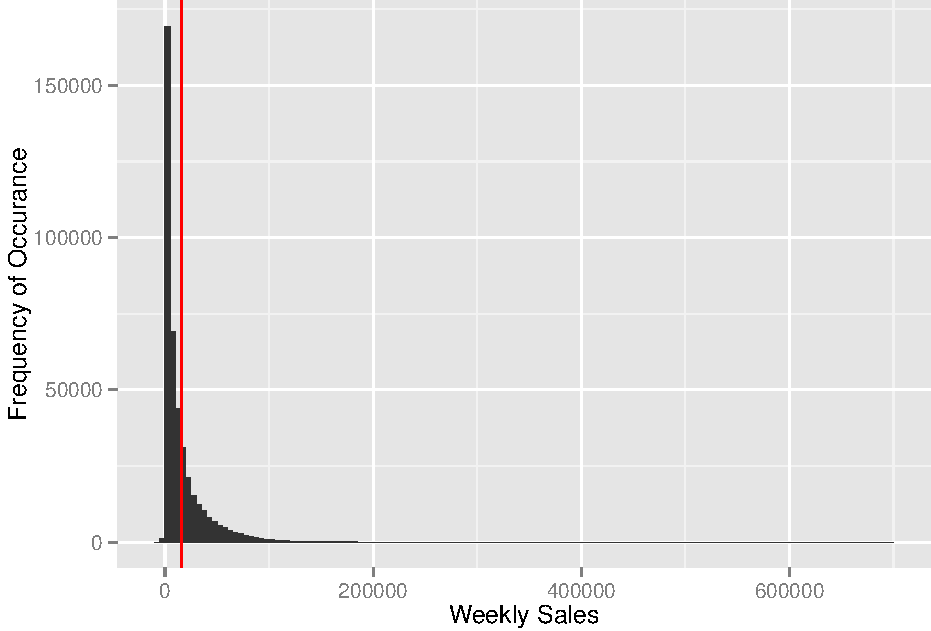
\includegraphics[width=400px]{PredictingWeeklySalesAtWalmart_files/figure-latex/weeklySalesSkew-1}

Since the data is highle skewed, it would be more appropriate use log
transformation to remove the skew to make make the data fit the
assumptions of inferential statistics. But before we do that, we need to
take care of Negative and Zero Values in the data.

\paragraph{3.1.1.2 Dealing with Negative and Zero Weekly
Sales}\label{dealing-with-negative-and-zero-weekly-sales}

Since Log transformation of negative numbers yeild NA and log
transformation of 0 is a negative infinity value, we need to handle
these values appropriately.

Let us first find the total count of numbers that fit this description:

\begin{Shaded}
\begin{Highlighting}[]
\NormalTok{## subsetting the values that are negative and 0}
\NormalTok{train0 <-}\StringTok{ }\KeywordTok{subset}\NormalTok{( train, train$Weekly_Sales <=}\StringTok{ }\DecValTok{0} \NormalTok{)}
\NormalTok{### Printing the first 5 rows of the data with negative and 0 values}
\KeywordTok{head}\NormalTok{( train0 )}
\end{Highlighting}
\end{Shaded}

\begin{verbatim}
##      Store Dept       Date Weekly_Sales IsHoliday
## 847      1    6 2012-08-10      -139.65     FALSE
## 2385     1   18 2012-05-04        -1.27     FALSE
## 6049     1   47 2010-02-19      -863.00     FALSE
## 6050     1   47 2010-03-12      -698.00     FALSE
## 6052     1   47 2010-10-08       -58.00     FALSE
## 6056     1   47 2011-03-11         0.00     FALSE
\end{verbatim}

\begin{itemize}
\itemsep1pt\parskip0pt\parsep0pt
\item
  The data set represents a paltry \texttt{0.3\%} of the full dataset -
  it has \texttt{1358} observations
\item
  The absolute sum of this Weekly\_Sales in this filtered data set is
  only \texttt{0.001\%} of the overall sum of Weekly\_Sales
\item
  The absolute maximum value of this dataset is \texttt{4988.94}
\end{itemize}

Owing to the reasons mentioned above, it would be good to remove these
observations from the dataset before continuting to do a Log
Transoformation of Weekly\_Sales.

\paragraph{3.1.1.3 Log Transformation of Weekly
Sales}\label{log-transformation-of-weekly-sales}

\begin{Shaded}
\begin{Highlighting}[]
\NormalTok{## Create subset of train data set}
\NormalTok{train <-}\StringTok{ }\KeywordTok{subset}\NormalTok{( train , train$Weekly_Sales >}\StringTok{ }\DecValTok{0} \NormalTok{)}
\NormalTok{## Make Log Transformation for Weekly_Sales}
\NormalTok{train$Log_Weekly_Sales <-}\StringTok{ }\KeywordTok{log}\NormalTok{(train$Weekly_Sales)}
\NormalTok{## remove train0}
\KeywordTok{rm}\NormalTok{( train0 )}
\end{Highlighting}
\end{Shaded}

\begin{verbatim}
## Warning in rm(train0): object 'train0' not found
\end{verbatim}

\begin{Shaded}
\begin{Highlighting}[]
\NormalTok{## summary statistics of Weekly_Sales and Log_Weekly_Sales}
\KeywordTok{summary}\NormalTok{(train$Weekly_Sales)}
\end{Highlighting}
\end{Shaded}

\begin{verbatim}
##    Min. 1st Qu.  Median    Mean 3rd Qu.    Max. 
##       0    2120    7662   16030   20270  693100
\end{verbatim}

\begin{Shaded}
\begin{Highlighting}[]
\KeywordTok{summary}\NormalTok{( train$Log_Weekly_Sales )}
\end{Highlighting}
\end{Shaded}

\begin{verbatim}
##    Min. 1st Qu.  Median    Mean 3rd Qu.    Max. 
##  -4.605   7.659   8.944   8.521   9.917  13.450
\end{verbatim}

We notice that the Median and the mean are more closer to teach other.
The histogram below shows that the data is less skewed than earlier:

\begin{Shaded}
\begin{Highlighting}[]
\NormalTok{## plotting the log( Weekly_Sales ) histogram}
\KeywordTok{ggplot}\NormalTok{( train, }\KeywordTok{aes}\NormalTok{( }\DataTypeTok{x =} \NormalTok{Log_Weekly_Sales ) ) +}
\StringTok{  }\KeywordTok{geom_histogram}\NormalTok{(}\DataTypeTok{binwidth=}\NormalTok{.}\DecValTok{2} \NormalTok{) +}\StringTok{ }
\StringTok{  }\NormalTok{## Vertical line indicating the mean value}
\StringTok{  }\KeywordTok{geom_vline}\NormalTok{( }\KeywordTok{aes}\NormalTok{( }\DataTypeTok{xintercept =} \KeywordTok{mean}\NormalTok{( Log_Weekly_Sales ) ), }\DataTypeTok{color=}\StringTok{"red"} \NormalTok{) +}
\StringTok{  }\KeywordTok{scale_y_continuous}\NormalTok{( }\StringTok{"Frequency of Occurance"} \NormalTok{) +}
\StringTok{  }\KeywordTok{scale_x_continuous}\NormalTok{( }\StringTok{"log( Weekly_Sales )"} \NormalTok{)}
\end{Highlighting}
\end{Shaded}

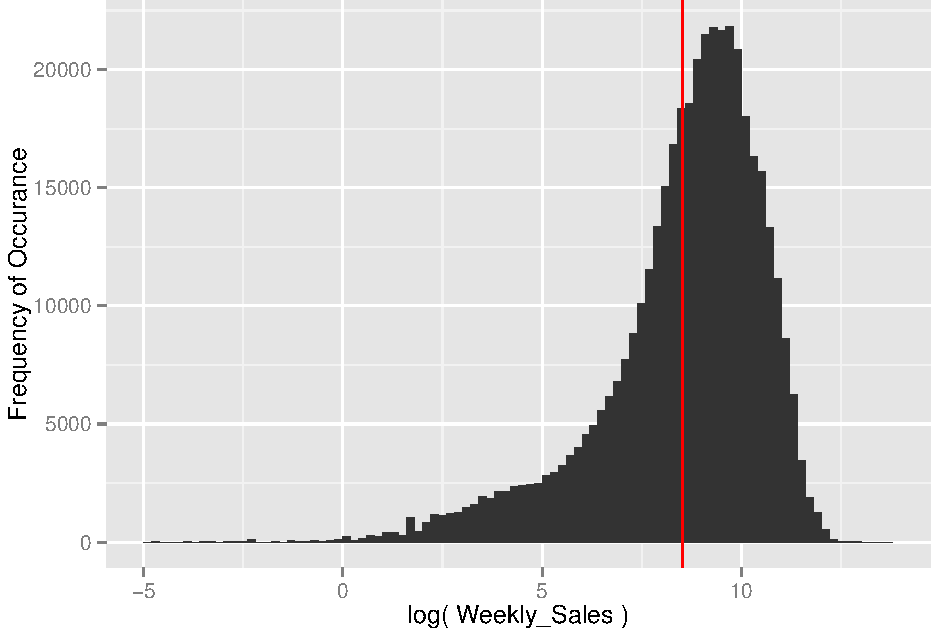
\includegraphics[width=400px]{PredictingWeeklySalesAtWalmart_files/figure-latex/logWeeklySalesHistogram-1}

The histogram is slightly \textbf{left-skewed}, but more normal than the
previous distribution of Weekly\_Sales.

\paragraph{3.1.1.4 Detailed Summary Statistics of Weekly
Sales}\label{detailed-summary-statistics-of-weekly-sales}

\begin{Shaded}
\begin{Highlighting}[]
\NormalTok{## Function to calculate the Standard Error}
\NormalTok{## x: the vector of numerical values}
\NormalTok{## returns the standard error of the vector}
\NormalTok{standardError <-}\StringTok{ }\NormalTok{function( x ) \{}
  \KeywordTok{sd}\NormalTok{( x )/}\KeywordTok{sqrt}\NormalTok{( }\KeywordTok{length}\NormalTok{( x ) )}
\NormalTok{\}}
\end{Highlighting}
\end{Shaded}

\begin{Shaded}
\begin{Highlighting}[]
\NormalTok{## Calculating Detailed Summary Statistics for Weekly_Sales}
\NormalTok{Weekly_Sales <-}\StringTok{ }\KeywordTok{c}\NormalTok{( }
  \KeywordTok{mean}\NormalTok{( train$Weekly_Sales ) ,}
  \KeywordTok{standardError}\NormalTok{(  train$Weekly_Sales ) ,}
  \KeywordTok{median}\NormalTok{( train$Weekly_Sales) ,}
  \KeywordTok{sd}\NormalTok{( train$Weekly_Sales ) ,}
  \KeywordTok{var}\NormalTok{( train$Weekly_Sales ) , }
  \KeywordTok{kurtosis}\NormalTok{( train$Weekly_Sales ) ,}
  \KeywordTok{skewness}\NormalTok{( train$Weekly_Sales ) ,}
  \KeywordTok{range}\NormalTok{( train$Weekly_Sales )[}\DecValTok{2}\NormalTok{]-}\KeywordTok{range}\NormalTok{( train$Weekly_Sales )[}\DecValTok{1}\NormalTok{] ,}
  \KeywordTok{min}\NormalTok{( train$Weekly_Sales ) ,}
  \KeywordTok{max}\NormalTok{( train$Weekly_Sales ) ,}
  \KeywordTok{sum}\NormalTok{( train$Weekly_Sales ),}
  \KeywordTok{length}\NormalTok{( train$Weekly_Sales ) }
\NormalTok{)}
\end{Highlighting}
\end{Shaded}

\begin{Shaded}
\begin{Highlighting}[]
\NormalTok{## Calculating Detailed Summary Statistics for Weekly_Sales}
\NormalTok{Log_Weekly_Sales <-}\StringTok{ }\KeywordTok{c}\NormalTok{( }
  \KeywordTok{mean}\NormalTok{( train$Log_Weekly_Sales ) ,}
  \KeywordTok{standardError}\NormalTok{(  train$Log_Weekly_Sales ) ,}
  \KeywordTok{median}\NormalTok{( train$Log_Weekly_Sales) ,}
  \KeywordTok{sd}\NormalTok{( train$Log_Weekly_Sales ) ,}
  \KeywordTok{var}\NormalTok{( train$Log_Weekly_Sales ) , }
  \KeywordTok{kurtosis}\NormalTok{( train$Log_Weekly_Sales ) ,}
  \KeywordTok{skewness}\NormalTok{( train$Log_Weekly_Sales ) ,}
  \KeywordTok{range}\NormalTok{( train$Log_Weekly_Sales )[}\DecValTok{2}\NormalTok{]-}\KeywordTok{range}\NormalTok{( train$Log_Weekly_Sales )[}\DecValTok{1}\NormalTok{] ,}
  \KeywordTok{min}\NormalTok{( train$Log_Weekly_Sales ) ,}
  \KeywordTok{max}\NormalTok{( train$Log_Weekly_Sales ) ,}
  \KeywordTok{sum}\NormalTok{( train$Log_Weekly_Sales ),}
  \KeywordTok{length}\NormalTok{( train$Log_Weekly_Sales ) }
\NormalTok{)}
\end{Highlighting}
\end{Shaded}

\begin{Shaded}
\begin{Highlighting}[]
\NormalTok{## Row Headings of the Summary statistics}
\NormalTok{Description <-}\StringTok{ }\KeywordTok{c}\NormalTok{(}
  \StringTok{"Mean"}\NormalTok{,}
  \StringTok{"Standard Error"} \NormalTok{,}
  \StringTok{"Median"} \NormalTok{, }
  \StringTok{"Standard Deviation"} \NormalTok{,}
  \StringTok{"Variance"} \NormalTok{, }
  \StringTok{"Kurtosis"} \NormalTok{,}
  \StringTok{"Skewness"} \NormalTok{,}
  \StringTok{"Range"} \NormalTok{,}
  \StringTok{"Min"} \NormalTok{,}
  \StringTok{"Max"} \NormalTok{,}
  \StringTok{"Sum"} \NormalTok{,}
  \StringTok{"Count"} 
\NormalTok{)}
\end{Highlighting}
\end{Shaded}

\begin{Shaded}
\begin{Highlighting}[]
\NormalTok{## Making a dataframe with the data}
\NormalTok{Detailed_Summary_Statistics_on_Weekly_Sales <-}\StringTok{ }
\StringTok{  }\KeywordTok{data.frame}\NormalTok{( }
    \DataTypeTok{Description=}\NormalTok{Description , }
    \DataTypeTok{Weekly_Sales =} \NormalTok{Weekly_Sales ,}
    \DataTypeTok{Log_Weekly_Sales =} \NormalTok{Log_Weekly_Sales}
    \NormalTok{)}
\NormalTok{## printing out the detailed summary statistics }
\KeywordTok{print}\NormalTok{( Detailed_Summary_Statistics_on_Weekly_Sales , }\DataTypeTok{row.names =} \NormalTok{F )}
\end{Highlighting}
\end{Shaded}

\begin{verbatim}
##         Description      Weekly_Sales  Log_Weekly_Sales
##                Mean      16033.114591       8.520815008
##      Standard Error         35.063520       0.003160895
##              Median       7661.700000       8.943989170
##  Standard Deviation      22729.492116       2.049010764
##            Variance  516629811.850102       4.198445111
##            Kurtosis         21.460407       2.221131837
##            Skewness          3.258918      -1.305705773
##               Range     693099.350000      18.054098831
##                 Min          0.010000      -4.605170186
##                 Max     693099.360000      13.448928645
##                 Sum 6737307148.670000 3580548.716211106
##               Count     420212.000000  420212.000000000
\end{verbatim}

\begin{Shaded}
\begin{Highlighting}[]
\NormalTok{## Removing intermediate data}
\KeywordTok{rm}\NormalTok{( }
  \NormalTok{Weekly_Sales ,  }
  \NormalTok{Log_Weekly_Sales , }
  \NormalTok{Description , }
  \NormalTok{Detailed_Summary_Statistics_on_Weekly_Sales )}
\end{Highlighting}
\end{Shaded}

The \textbf{Kurtosis} value of Log\_Weekly\_Sales indicates that it is
peaked - unimodal data.

\subsubsection{3.1.2 The Stores Dataset
(stores)}\label{the-stores-dataset-stores}

\begin{Shaded}
\begin{Highlighting}[]
\NormalTok{## Structure of Stores Dataset}
\KeywordTok{str}\NormalTok{(stores)}
\end{Highlighting}
\end{Shaded}

\begin{verbatim}
## 'data.frame':    45 obs. of  3 variables:
##  $ Store: int  1 2 3 4 5 6 7 8 9 10 ...
##  $ Type : Factor w/ 3 levels "A","B","C": 1 1 2 1 2 1 2 1 2 2 ...
##  $ Size : int  151315 202307 37392 205863 34875 202505 70713 155078 125833 126512 ...
\end{verbatim}

\begin{Shaded}
\begin{Highlighting}[]
\NormalTok{## summary Statistics of Stores dataset}
\KeywordTok{summary}\NormalTok{(stores)}
\end{Highlighting}
\end{Shaded}

\begin{verbatim}
##      Store    Type        Size       
##  Min.   : 1   A:22   Min.   : 34875  
##  1st Qu.:12   B:17   1st Qu.: 70713  
##  Median :23   C: 6   Median :126512  
##  Mean   :23          Mean   :130288  
##  3rd Qu.:34          3rd Qu.:202307  
##  Max.   :45          Max.   :219622
\end{verbatim}

No missing data.

The stores are grouped into types, and it appears to be mostly a
function of its size. The following boxplot indicates this:

\begin{Shaded}
\begin{Highlighting}[]
\NormalTok{## box plot to show the summary statistics of the Type of Stores and their sizes}
\KeywordTok{ggplot}\NormalTok{(}\DataTypeTok{data=}\NormalTok{stores, }
       \KeywordTok{aes}\NormalTok{(}\DataTypeTok{x=}\NormalTok{Type, }\DataTypeTok{y=}\NormalTok{Size, }\DataTypeTok{fill=}\NormalTok{Type) ) +}\StringTok{ }
\StringTok{  }\KeywordTok{geom_boxplot}\NormalTok{(}\DataTypeTok{outlier.shape =} \DecValTok{15}\NormalTok{, }\DataTypeTok{outlier.size =} \DecValTok{4}\NormalTok{) +}
\StringTok{  }\NormalTok{## to show how the individual store sizes are distributed}
\StringTok{  }\KeywordTok{geom_jitter}\NormalTok{() +}
\StringTok{  }\KeywordTok{scale_y_continuous}\NormalTok{( }\DataTypeTok{name=}\StringTok{"Store Size"} \NormalTok{) +}\StringTok{ }
\StringTok{  }\KeywordTok{scale_fill_brewer}\NormalTok{( }\DataTypeTok{name =} \StringTok{"Store Type"} \NormalTok{, }\DataTypeTok{palette =} \StringTok{"Dark2"}\NormalTok{)}
\end{Highlighting}
\end{Shaded}

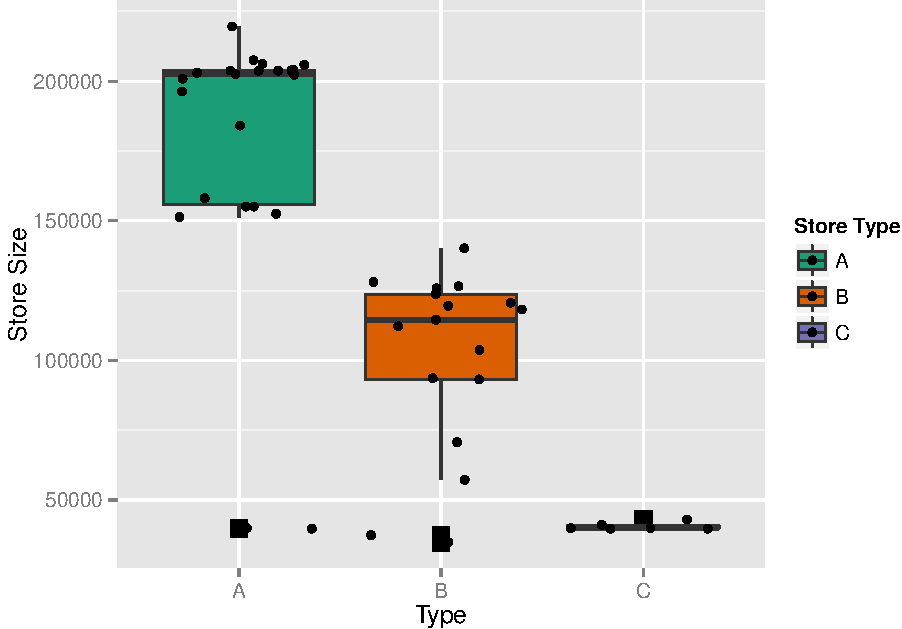
\includegraphics[width=400px]{PredictingWeeklySalesAtWalmart_files/figure-latex/storeSizeBoxPlot-1}

\begin{Shaded}
\begin{Highlighting}[]
\NormalTok{## Standard Deviation of each type of Store}
\KeywordTok{tapply}\NormalTok{( stores$Size , stores$Type , sd )}
\end{Highlighting}
\end{Shaded}

\begin{verbatim}
##         A         B         C 
## 49392.621 32371.138  1304.145
\end{verbatim}

\begin{Shaded}
\begin{Highlighting}[]
\NormalTok{## Median of each Type of Store}
\KeywordTok{tapply}\NormalTok{( stores$Size , stores$Type , median )}
\end{Highlighting}
\end{Shaded}

\begin{verbatim}
##      A      B      C 
## 202406 114533  39910
\end{verbatim}

\begin{Shaded}
\begin{Highlighting}[]
\NormalTok{## Mean of each type of Store}
\KeywordTok{tapply}\NormalTok{( stores$Size , stores$Type , mean )}
\end{Highlighting}
\end{Shaded}

\begin{verbatim}
##         A         B         C 
## 177247.73 101190.71  40541.67
\end{verbatim}

\subsubsection{3.1.3 The Features Dataset
(features)}\label{the-features-dataset-features}

\begin{Shaded}
\begin{Highlighting}[]
\NormalTok{## Structure of features dataset}
\KeywordTok{str}\NormalTok{(features)}
\end{Highlighting}
\end{Shaded}

\begin{verbatim}
## 'data.frame':    8190 obs. of  12 variables:
##  $ Store       : int  1 1 1 1 1 1 1 1 1 1 ...
##  $ Date        : Factor w/ 182 levels "2010-02-05","2010-02-12",..: 1 2 3 4 5 6 7 8 9 10 ...
##  $ Temperature : num  42.3 38.5 39.9 46.6 46.5 ...
##  $ Fuel_Price  : num  2.57 2.55 2.51 2.56 2.62 ...
##  $ MarkDown1   : num  NA NA NA NA NA NA NA NA NA NA ...
##  $ MarkDown2   : num  NA NA NA NA NA NA NA NA NA NA ...
##  $ MarkDown3   : num  NA NA NA NA NA NA NA NA NA NA ...
##  $ MarkDown4   : num  NA NA NA NA NA NA NA NA NA NA ...
##  $ MarkDown5   : num  NA NA NA NA NA NA NA NA NA NA ...
##  $ CPI         : num  211 211 211 211 211 ...
##  $ Unemployment: num  8.11 8.11 8.11 8.11 8.11 ...
##  $ IsHoliday   : logi  FALSE TRUE FALSE FALSE FALSE FALSE ...
\end{verbatim}

Date is ingested as factor (as opposed to being ingested as date type).
There are 182 dates in total. This data set is relevant for both the
train and the test data set.

\begin{Shaded}
\begin{Highlighting}[]
\NormalTok{## Changing the Date from "Format" type to "Date" Type }
\NormalTok{features$Date <-}\StringTok{ }\KeywordTok{as.Date}\NormalTok{(features$Date)}
\NormalTok{## Summary Statistics of Features Dataset}
\KeywordTok{summary}\NormalTok{(features)}
\end{Highlighting}
\end{Shaded}

\begin{verbatim}
##      Store         Date             Temperature       Fuel_Price   
##  Min.   : 1   Min.   :2010-02-05   Min.   : -7.29   Min.   :2.472  
##  1st Qu.:12   1st Qu.:2010-12-17   1st Qu.: 45.90   1st Qu.:3.041  
##  Median :23   Median :2011-10-31   Median : 60.71   Median :3.513  
##  Mean   :23   Mean   :2011-10-31   Mean   : 59.36   Mean   :3.406  
##  3rd Qu.:34   3rd Qu.:2012-09-14   3rd Qu.: 73.88   3rd Qu.:3.743  
##  Max.   :45   Max.   :2013-07-26   Max.   :101.95   Max.   :4.468  
##                                                                    
##    MarkDown1        MarkDown2           MarkDown3           MarkDown4       
##  Min.   : -2781   Min.   :  -265.76   Min.   :  -179.26   Min.   :    0.22  
##  1st Qu.:  1578   1st Qu.:    68.88   1st Qu.:     6.60   1st Qu.:  304.69  
##  Median :  4744   Median :   364.57   Median :    36.26   Median : 1176.42  
##  Mean   :  7032   Mean   :  3384.18   Mean   :  1760.10   Mean   : 3292.94  
##  3rd Qu.:  8923   3rd Qu.:  2153.35   3rd Qu.:   163.15   3rd Qu.: 3310.01  
##  Max.   :103185   Max.   :104519.54   Max.   :149483.31   Max.   :67474.85  
##  NA's   :4158     NA's   :5269        NA's   :4577        NA's   :4726      
##    MarkDown5             CPI         Unemployment    IsHoliday      
##  Min.   :  -185.2   Min.   :126.1   Min.   : 3.684   Mode :logical  
##  1st Qu.:  1440.8   1st Qu.:132.4   1st Qu.: 6.634   FALSE:7605     
##  Median :  2727.1   Median :182.8   Median : 7.806   TRUE :585      
##  Mean   :  4132.2   Mean   :172.5   Mean   : 7.827   NA's :0        
##  3rd Qu.:  4832.6   3rd Qu.:213.9   3rd Qu.: 8.567                  
##  Max.   :771448.1   Max.   :229.0   Max.   :14.313                  
##  NA's   :4140       NA's   :585     NA's   :585
\end{verbatim}

The features data set has missing variables for Markdown1-5, CPI \&
Unemployment. We will discuss how we can treat these missing values
below

\paragraph{3.1.3.1 Handling Consumer Price Index Missing
Values}\label{handling-consumer-price-index-missing-values}

To undertstand how the missing values are distributed in the features
dataset let us first plot a heat map.

\begin{Shaded}
\begin{Highlighting}[]
\NormalTok{## Calculating the mean CPI Across all the stores by Date}
\NormalTok{meanCPIAcrossStores <-}\StringTok{ }\KeywordTok{tapply}\NormalTok{( features$CPI , features$Date , }\DataTypeTok{FUN =} \NormalTok{mean )}
\NormalTok{## Converting it into Data Frame}
\NormalTok{meanCPIAcrossStoresDF <-}\StringTok{ }\KeywordTok{data.frame}\NormalTok{( meanCPIAcrossStores )}
\NormalTok{## Adding the row Data to the data frame to see the trend}
\NormalTok{meanCPIAcrossStoresDF$Date <-}\StringTok{ }\KeywordTok{as.Date}\NormalTok{( }\KeywordTok{rownames}\NormalTok{( meanCPIAcrossStoresDF ) )}
\end{Highlighting}
\end{Shaded}

\begin{Shaded}
\begin{Highlighting}[]
\NormalTok{## heatmap to undersatnd where CPI is missing}
\NormalTok{missingCPIHeatMap <-}\StringTok{ }\KeywordTok{ggplot}\NormalTok{( features , }\KeywordTok{aes}\NormalTok{(}\DataTypeTok{x =} \NormalTok{Date, }\DataTypeTok{y =} \NormalTok{Store)) +}\StringTok{ }
\StringTok{  }\KeywordTok{geom_tile}\NormalTok{(}\KeywordTok{aes}\NormalTok{(}\DataTypeTok{fill =} \NormalTok{CPI)) +}
\StringTok{  }\KeywordTok{scale_fill_gradient}\NormalTok{(}\DataTypeTok{low=}\StringTok{"yellow"}\NormalTok{, }\DataTypeTok{high=}\StringTok{"red"} \NormalTok{, }\DataTypeTok{labels =} \NormalTok{comma , }\DataTypeTok{name=}\StringTok{"CPI"}\NormalTok{) +}
\StringTok{  }\KeywordTok{scale_y_continuous}\NormalTok{(}\DataTypeTok{name=}\StringTok{"Store"}\NormalTok{) +}
\StringTok{  }\KeywordTok{theme}\NormalTok{( }\DataTypeTok{legend.position =} \StringTok{"none"} \NormalTok{)}
\NormalTok{## trend of Average CPI Across All Stores}
\NormalTok{avgCPiIndexTrend <-}\StringTok{ }\KeywordTok{ggplot}\NormalTok{( meanCPIAcrossStoresDF , }\KeywordTok{aes}\NormalTok{(}\DataTypeTok{x =} \NormalTok{Date, }\DataTypeTok{y =} \NormalTok{meanCPIAcrossStores ) ) +}\StringTok{ }
\StringTok{  }\KeywordTok{geom_line}\NormalTok{() +}
\StringTok{  }\KeywordTok{scale_y_continuous}\NormalTok{(}\DataTypeTok{name=}\StringTok{"MEAN CPI Across All Stores"} \NormalTok{) +}
\StringTok{  }\NormalTok{## Adding a linear model to view the trend}
\StringTok{  }\KeywordTok{stat_smooth}\NormalTok{( }\DataTypeTok{method =} \StringTok{"lm"} \NormalTok{)}
\NormalTok{## putting the graphs into a grid}
\KeywordTok{grid.arrange}\NormalTok{(missingCPIHeatMap , avgCPiIndexTrend , }\DataTypeTok{ncol =} \DecValTok{1} \NormalTok{)}
\end{Highlighting}
\end{Shaded}

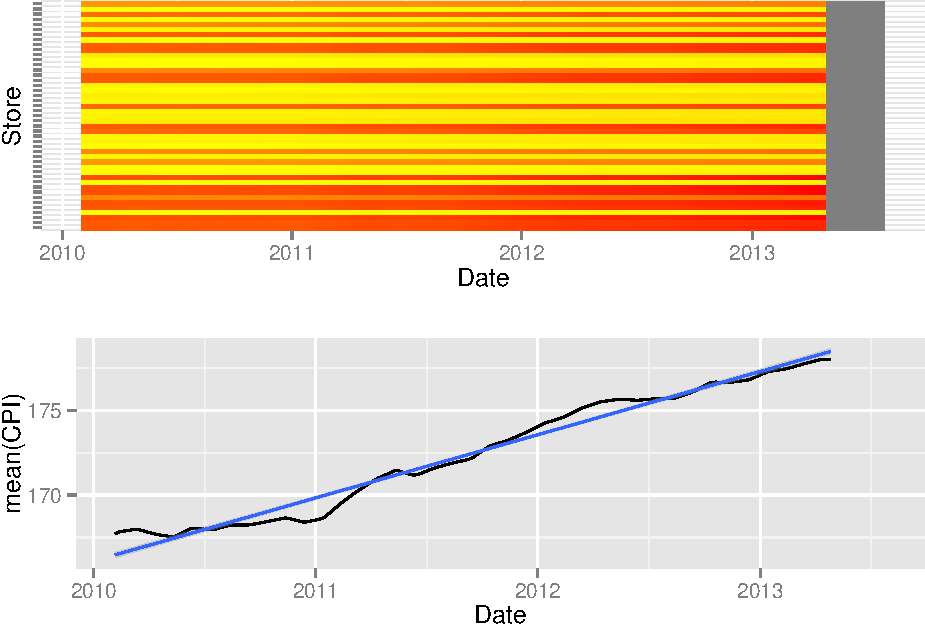
\includegraphics[width=400px]{PredictingWeeklySalesAtWalmart_files/figure-latex/CPIMissingHeatMap-1}

The following features stand out:

\begin{itemize}
\itemsep1pt\parskip0pt\parsep0pt
\item
  Data for CPI is missing a little after mid-2013
\item
  There is high variation of CPI between different stores
\item
  But the variation over time is minimal - as the colors on the heat map
  suggest - which stays constant
\item
  Taking an average CPI across all stores, we notice an upward trend
\end{itemize}

It is not feasible to fetch the missing CPI Value for anonymised stores,
therefore, we will build a linear model to predict the CPI Value for the
missing values.

\begin{Shaded}
\begin{Highlighting}[]
\NormalTok{## CPI MEAN, MAX MIN & Range tabulated into a Data Frame}
\NormalTok{CPI_Mean <-}\StringTok{ }\KeywordTok{tapply}\NormalTok{( features$CPI , features$Store , }\DataTypeTok{FUN =} \NormalTok{mean , }\DataTypeTok{na.rm=} \NormalTok{T )}
\NormalTok{CPI_Max <-}\StringTok{ }\KeywordTok{tapply}\NormalTok{( features$CPI , features$Store , }\DataTypeTok{FUN =} \NormalTok{mean , }\DataTypeTok{na.rm=} \NormalTok{T )}
\NormalTok{CPI_Min <-}\StringTok{ }\KeywordTok{tapply}\NormalTok{( features$CPI , features$Store , }\DataTypeTok{FUN =} \NormalTok{mean , }\DataTypeTok{na.rm=} \NormalTok{T )}
\NormalTok{CPI_DF <-}\StringTok{ }\KeywordTok{data.frame}\NormalTok{( CPI_Mean , CPI_Max , CPI_Min )}
\NormalTok{CPI_DF$Range <-}\StringTok{ }\NormalTok{CPI_DF$CPI_Max -}\StringTok{ }\NormalTok{CPI_DF$CPI_Min }
\NormalTok{## Checking if there is a difference between Max and Min}
\NormalTok{## - if no change then no rows}
\NormalTok{CPI_DF[ CPI_DF$Range !=}\StringTok{ }\DecValTok{0} \NormalTok{,]}
\end{Highlighting}
\end{Shaded}

\begin{verbatim}
## [1] CPI_Mean CPI_Max  CPI_Min  Range   
## <0 rows> (or 0-length row.names)
\end{verbatim}

While checking if there was any variation for CPI, we find that there
are no rows. This indicates that there is no variation in CPI and we can
confidently impute the missing values of CPI to each store's specific
CPI.

\begin{Shaded}
\begin{Highlighting}[]
\NormalTok{## Removing CPI Columns not needed anymore}
\NormalTok{CPI_DF$CPI_Min =}\StringTok{ }\NormalTok{CPI_DF$CPI_Max =}\StringTok{ }\NormalTok{CPI_DF$Range =}\StringTok{ }\OtherTok{NULL}
\NormalTok{## Creating Store Column with the RowNAME}
\NormalTok{CPI_DF$Store <-}\StringTok{ }\KeywordTok{as.integer}\NormalTok{( }\KeywordTok{rownames}\NormalTok{( CPI_DF ) )}
\NormalTok{## Imputing CPI}
\NormalTok{## merging the dataframes by Store}
\NormalTok{features1 <-}\StringTok{ }\KeywordTok{merge}\NormalTok{( features , CPI_DF , }\DataTypeTok{by=}\StringTok{"Store"} \NormalTok{)}
\NormalTok{## removing old CPI Column}
\NormalTok{features1$CPI =}\StringTok{ }\OtherTok{NULL}
\NormalTok{## Renaming CPI_Mean to CPI - it is the last column in the data frame}
\KeywordTok{colnames}\NormalTok{( features1 )[ }\KeywordTok{ncol}\NormalTok{( features1 ) ] <-}\StringTok{ "CPI"}
\end{Highlighting}
\end{Shaded}

Let us visually verify if CPI data was imputed correctly

\begin{Shaded}
\begin{Highlighting}[]
\NormalTok{## checking if the imputation was done correctly}
\NormalTok{newCPIHeatMap <-}\StringTok{ }\KeywordTok{ggplot}\NormalTok{( features1 , }\KeywordTok{aes}\NormalTok{(}\DataTypeTok{x =} \NormalTok{Date, }\DataTypeTok{y =} \NormalTok{Store)) +}\StringTok{ }
\StringTok{  }\KeywordTok{geom_tile}\NormalTok{(}\KeywordTok{aes}\NormalTok{(}\DataTypeTok{fill =} \NormalTok{CPI)) +}
\StringTok{  }\KeywordTok{scale_fill_gradient}\NormalTok{(}\DataTypeTok{low=}\StringTok{"yellow"}\NormalTok{, }\DataTypeTok{high=}\StringTok{"red"} \NormalTok{, }\DataTypeTok{labels =} \NormalTok{comma , }\DataTypeTok{name=}\StringTok{"CPI"}\NormalTok{) +}
\StringTok{  }\KeywordTok{scale_y_continuous}\NormalTok{(}\DataTypeTok{name=}\StringTok{"Store"}\NormalTok{) +}
\StringTok{  }\KeywordTok{theme}\NormalTok{( }\DataTypeTok{legend.position =} \StringTok{"none"} \NormalTok{)}
\NormalTok{## arranging both the old and new graphs in a grid}
\KeywordTok{grid.arrange}\NormalTok{( missingCPIHeatMap , newCPIHeatMap , }\DataTypeTok{ncol =} \DecValTok{1} \NormalTok{)}
\end{Highlighting}
\end{Shaded}

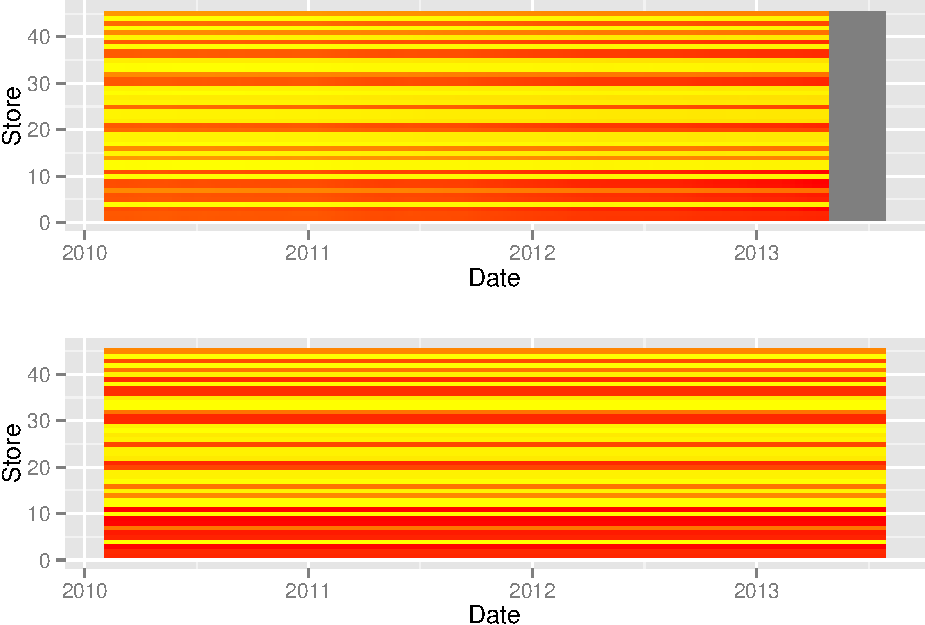
\includegraphics[width=400px]{PredictingWeeklySalesAtWalmart_files/figure-latex/plottingNewCPI-1}

\begin{Shaded}
\begin{Highlighting}[]
\NormalTok{## overwriting old features with features1 (with no missing values for CPI)}
\NormalTok{features <-}\StringTok{ }\NormalTok{features1}
\NormalTok{## removing unneccesary data elements}
\KeywordTok{rm}\NormalTok{( CPI_DF , CPI_Max , CPI_Mean , CPI_Min , }
    \NormalTok{features1 , newCPIHeatMap , missingCPIHeatMap ,}
    \NormalTok{meanCPIAcrossStores , meanCPIAcrossStoresDF , avgCPiIndexTrend )}
\end{Highlighting}
\end{Shaded}

\subsubsection{3.1.4 The Test Dataset
(test)}\label{the-test-dataset-test}

\begin{Shaded}
\begin{Highlighting}[]
\NormalTok{## Structure of test dataset}
\KeywordTok{str}\NormalTok{(test)}
\end{Highlighting}
\end{Shaded}

\begin{verbatim}
## 'data.frame':    115064 obs. of  4 variables:
##  $ Store    : int  1 1 1 1 1 1 1 1 1 1 ...
##  $ Dept     : int  1 1 1 1 1 1 1 1 1 1 ...
##  $ Date     : Factor w/ 39 levels "2012-11-02","2012-11-09",..: 1 2 3 4 5 6 7 8 9 10 ...
##  $ IsHoliday: logi  FALSE FALSE FALSE TRUE FALSE FALSE ...
\end{verbatim}

Date is ingested as factor (as opposed to being ingested as date type).
There are 39 dates in total.

\begin{Shaded}
\begin{Highlighting}[]
\NormalTok{## Changing the Date from "Format" type to "Date" Type }
\NormalTok{test$Date <-}\StringTok{ }\KeywordTok{as.Date}\NormalTok{(test$Date)}
\NormalTok{## Summary Statistics of test Dataset}
\KeywordTok{summary}\NormalTok{(test)}
\end{Highlighting}
\end{Shaded}

\begin{verbatim}
##      Store            Dept            Date            IsHoliday      
##  Min.   : 1.00   Min.   : 1.00   Min.   :2012-11-02   Mode :logical  
##  1st Qu.:11.00   1st Qu.:18.00   1st Qu.:2013-01-04   FALSE:106136   
##  Median :22.00   Median :37.00   Median :2013-03-15   TRUE :8928     
##  Mean   :22.24   Mean   :44.34   Mean   :2013-03-14   NA's :0        
##  3rd Qu.:33.00   3rd Qu.:74.00   3rd Qu.:2013-05-24                  
##  Max.   :45.00   Max.   :99.00   Max.   :2013-07-26
\end{verbatim}

\pagebreak

\subsection{3.2 Data Preparation - Merging the
Datasets}\label{data-preparation---merging-the-datasets}

\subsubsection{3.2.1 Merging Train and Stores
Datasets}\label{merging-train-and-stores-datasets}

Since the Type \& Size variables may influence the Weekly Sales, we are
merging the train \& data sets. We merge the data by Store.

\begin{Shaded}
\begin{Highlighting}[]
\NormalTok{## Merging train and stores by Store}
\NormalTok{trainStoresMerge <-}\StringTok{ }\KeywordTok{merge}\NormalTok{(train , stores , }\DataTypeTok{by =} \StringTok{"Store"}\NormalTok{)}
\end{Highlighting}
\end{Shaded}

\subsubsection{3.2.2 Merging Train, Stores and Features
Datasets}\label{merging-train-stores-and-features-datasets}

Since Markdown1-5 and other variables could play an important role at
predicting Weekly\_Sales, this should be merged with the
trainStoresMerge data set. We merge the data by Store \& Date.

\begin{Shaded}
\begin{Highlighting}[]
\NormalTok{## Merging trainStoresMerge and features datasets}
\NormalTok{trainStoresFeaturesMerge <-}\StringTok{ }
\StringTok{  }\KeywordTok{merge}\NormalTok{( trainStoresMerge , features , }\DataTypeTok{by =} \KeywordTok{c}\NormalTok{( }\StringTok{"Store"} \NormalTok{, }\StringTok{"Date"} \NormalTok{) )}
\NormalTok{## Clearing memory - removing intermediate datasets}
\KeywordTok{rm}\NormalTok{( trainStoresMerge )}
\NormalTok{## Fixing the name of the Column}
\KeywordTok{colnames}\NormalTok{(trainStoresFeaturesMerge)[}\DecValTok{5}\NormalTok{] <-}\StringTok{ "IsHoliday"}
\NormalTok{trainStoresFeaturesMerge$IsHoliday.y <-}\StringTok{ }\OtherTok{NULL}
\end{Highlighting}
\end{Shaded}

\subsubsection{3.2.3 Merging Test, Stores and Features
Datasets}\label{merging-test-stores-and-features-datasets}

We similarly merge the test, stores \& features to create the
testStoresFeaturesMerge data set.

\begin{Shaded}
\begin{Highlighting}[]
\NormalTok{## Merging test and stores by Store}
\NormalTok{testStoresMerge <-}\StringTok{ }\KeywordTok{merge}\NormalTok{(test , stores , }\DataTypeTok{by =} \StringTok{"Store"}\NormalTok{)}
\NormalTok{## Merging testStoresMerge and features datasets}
\NormalTok{testStoresFeaturesMerge <-}\StringTok{ }
\StringTok{  }\KeywordTok{merge}\NormalTok{( testStoresMerge , features , }\DataTypeTok{by =} \KeywordTok{c}\NormalTok{( }\StringTok{"Store"} \NormalTok{, }\StringTok{"Date"} \NormalTok{) )}
\NormalTok{## Clearing Memory - removing intermediate Datasets}
\KeywordTok{rm}\NormalTok{( testStoresMerge )}
\NormalTok{## Fixing the name of the Column}
\KeywordTok{colnames}\NormalTok{(testStoresFeaturesMerge)[}\DecValTok{5}\NormalTok{] <-}\StringTok{ "IsHoliday"}
\NormalTok{testStoresFeaturesMerge$IsHoliday.y <-}\StringTok{ }\OtherTok{NULL}
\end{Highlighting}
\end{Shaded}

\pagebreak

\subsection{3.3 Data Exploration}\label{data-exploration}

\subsubsection{3.3.1 Total Sales Per Department in each
Store}\label{total-sales-per-department-in-each-store}

The final goal of this report is to be able to predict the weekly sales
for each department in a store. First we would like to understand which
departments are present in the 45 different stores and their total
sales.

\begin{Shaded}
\begin{Highlighting}[]
\NormalTok{## running the sum function for each store & department}
\NormalTok{storeDeptTotalSales <-}\StringTok{ }\KeywordTok{tapply}\NormalTok{( }
  \NormalTok{trainStoresFeaturesMerge$Weekly_Sales , }
  \NormalTok{trainStoresFeaturesMerge[, }\KeywordTok{c}\NormalTok{(}\StringTok{"Store"}\NormalTok{,}\StringTok{"Dept"}\NormalTok{)]  , }
  \DataTypeTok{FUN =} \NormalTok{sum )}
\NormalTok{## Converting the matrix to a dataframe}
\NormalTok{storeDeptTotalSalesDataFrame <-}\StringTok{ }\KeywordTok{as.data.frame}\NormalTok{( storeDeptTotalSales )}
\NormalTok{## Setting the Store Number into the table so we can analyze it further}
\NormalTok{storeDeptTotalSalesDataFrame$Store <-}\StringTok{ }
\StringTok{  }\KeywordTok{as.integer}\NormalTok{( }\KeywordTok{rownames}\NormalTok{( storeDeptTotalSalesDataFrame ) )}
\NormalTok{## Move Store to the 1st column in the dataframe}
\NormalTok{storeDeptTotalSalesDataFrame <-}\StringTok{ }
\StringTok{  }\NormalTok{storeDeptTotalSalesDataFrame[ , }\KeywordTok{c}\NormalTok{( }\KeywordTok{ncol}\NormalTok{(storeDeptTotalSalesDataFrame) , }\DecValTok{1}\NormalTok{:}\KeywordTok{ncol}\NormalTok{(storeDeptTotalSalesDataFrame)-}\DecValTok{1} \NormalTok{)]}
\NormalTok{## Melting the columns into rows to enable analysis}
\NormalTok{storeDeptTotalSalesDataFrame <-}\StringTok{ }
\StringTok{  }\KeywordTok{melt}\NormalTok{(storeDeptTotalSalesDataFrame , }\DataTypeTok{id=}\StringTok{"Store"} \NormalTok{)}
\NormalTok{## removing the NA variables - where the department does not exist in a store}
\NormalTok{storeDeptTotalSalesDataFrame <-}\StringTok{ }\NormalTok{storeDeptTotalSalesDataFrame[ }\KeywordTok{complete.cases}\NormalTok{(storeDeptTotalSalesDataFrame),]}
\NormalTok{## Renaming the Columns in the Dataframe}
\KeywordTok{colnames}\NormalTok{( storeDeptTotalSalesDataFrame )[}\DecValTok{2}\NormalTok{:}\DecValTok{3}\NormalTok{] <-}\StringTok{ }\KeywordTok{c}\NormalTok{(}\StringTok{"Dept"} \NormalTok{, }\StringTok{"TotalSales"} \NormalTok{)}
\NormalTok{## Changing the Dept Type from String to Numeric}
\NormalTok{storeDeptTotalSalesDataFrame$Dept <-}\StringTok{ }
\StringTok{  }\KeywordTok{as.integer}\NormalTok{(storeDeptTotalSalesDataFrame$Dept)}
\NormalTok{## printing out summary statistics}
\KeywordTok{summary}\NormalTok{( storeDeptTotalSalesDataFrame)}
\end{Highlighting}
\end{Shaded}

\begin{verbatim}
##      Store            Dept         TotalSales      
##  Min.   : 1.00   Min.   : 1.00   Min.   :       0  
##  1st Qu.:11.00   1st Qu.:19.00   1st Qu.:  142430  
##  Median :22.00   Median :40.00   Median :  884694  
##  Mean   :22.47   Mean   :40.48   Mean   : 2027477  
##  3rd Qu.:33.00   3rd Qu.:62.00   3rd Qu.: 2623710  
##  Max.   :45.00   Max.   :81.00   Max.   :26101498
\end{verbatim}

\begin{Shaded}
\begin{Highlighting}[]
\NormalTok{## Freeing Memory}
\KeywordTok{rm}\NormalTok{( storeDeptTotalSales )}
\end{Highlighting}
\end{Shaded}

\paragraph{3.3.1.1 Heat Map - Store \& Department Total
Sales}\label{heat-map---store-department-total-sales}

We generate a heat map to study this interaction

\begin{Shaded}
\begin{Highlighting}[]
\NormalTok{## Generating a Heatmap of the Department's Total Sales in each of 45 stores}
\KeywordTok{ggplot}\NormalTok{( storeDeptTotalSalesDataFrame , }\KeywordTok{aes}\NormalTok{(}\DataTypeTok{x =} \NormalTok{Store, }\DataTypeTok{y =} \NormalTok{Dept)) +}\StringTok{ }
\StringTok{  }\KeywordTok{geom_tile}\NormalTok{(}\KeywordTok{aes}\NormalTok{(}\DataTypeTok{fill =} \NormalTok{TotalSales)) +}
\StringTok{  }\KeywordTok{scale_fill_gradient}\NormalTok{(}
    \DataTypeTok{low=}\StringTok{"yellow"}\NormalTok{, }\DataTypeTok{high=}\StringTok{"red"} \NormalTok{, }\DataTypeTok{labels =} \NormalTok{comma , }\DataTypeTok{name=}\StringTok{"Total Sales"}\NormalTok{) +}
\StringTok{  }\KeywordTok{scale_y_continuous}\NormalTok{(}\DataTypeTok{name=}\StringTok{"Department"}\NormalTok{)}
\end{Highlighting}
\end{Shaded}

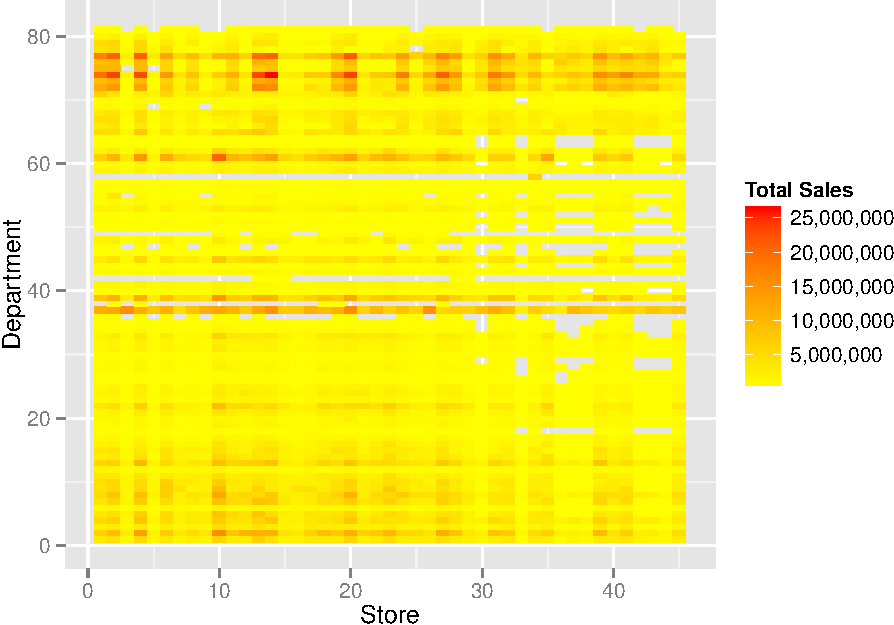
\includegraphics[width=400px]{PredictingWeeklySalesAtWalmart_files/figure-latex/heatmapStoreDept-1}
From the heat map we can draw the following broad conclusions:

\begin{itemize}
\itemsep1pt\parskip0pt\parsep0pt
\item
  The departments between 70-80 account for more sales than other
  departments
\item
  Some departments are missing in some stores
\end{itemize}

\begin{Shaded}
\begin{Highlighting}[]
\NormalTok{## removing dataframe to free up memory}
\KeywordTok{rm}\NormalTok{( storeDeptTotalSalesDataFrame )}
\end{Highlighting}
\end{Shaded}

\subsubsection{3.3.2 Store Total Sales Vs.
Size}\label{store-total-sales-vs.-size}

Plotting the total sales of a store vs.~Store Size. We first calculate
the total sales per Store and plot it as a response (y-axis) to the
Store size (x-axis) to understand the relationship between them.

\begin{Shaded}
\begin{Highlighting}[]
\NormalTok{## Total Sales vs. Store Size - plotting the relationship}
\NormalTok{## calculating the sum of all the store sales}
\NormalTok{StoreTotalSales <-}\StringTok{ }
\StringTok{  }\KeywordTok{tapply}\NormalTok{(}
    \NormalTok{trainStoresFeaturesMerge$Weekly_Sales, }
    \NormalTok{trainStoresFeaturesMerge$Store, }
    \DataTypeTok{FUN =} \NormalTok{sum)}
\NormalTok{## converting the table to a DataFrame}
\NormalTok{stores$TotalSales <-}\StringTok{ }\NormalTok{StoreTotalSales}
\NormalTok{stores$TotalSalesInMillion <-}\StringTok{ }\NormalTok{stores$TotalSales/}\DecValTok{1000000}
\KeywordTok{rm}\NormalTok{( StoreTotalSales )}
\end{Highlighting}
\end{Shaded}

\begin{Shaded}
\begin{Highlighting}[]
\NormalTok{## Plotting the Total Sales vs. Store Size}
\NormalTok{scatterPlotStoreSize <-}\StringTok{ }\KeywordTok{ggplot}\NormalTok{( stores , }\KeywordTok{aes}\NormalTok{(}\DataTypeTok{x=}\NormalTok{Size , }\DataTypeTok{y=}\NormalTok{TotalSalesInMillion , }\DataTypeTok{color =} \NormalTok{Type ) ) +}\StringTok{ }
\StringTok{  }\KeywordTok{geom_point}\NormalTok{( }\DataTypeTok{size=}\DecValTok{3}\NormalTok{) +}\StringTok{  }
\StringTok{  }\KeywordTok{scale_y_continuous}\NormalTok{(}\DataTypeTok{name=}\StringTok{"Total Sales in Millions"} \NormalTok{) +}\StringTok{ }
\StringTok{  }\KeywordTok{scale_color_brewer}\NormalTok{(}\DataTypeTok{palette =} \StringTok{"Dark2"}\NormalTok{, }\DataTypeTok{name=}\StringTok{"Store Type"} \NormalTok{) +}
\StringTok{  }\KeywordTok{theme}\NormalTok{( }\DataTypeTok{legend.position =} \StringTok{"bottom"} \NormalTok{)}
\end{Highlighting}
\end{Shaded}

\begin{Shaded}
\begin{Highlighting}[]
\NormalTok{## box plot to show the summary statistics of the Type of Stores}
\NormalTok{boxplotStoreSize <-}\StringTok{ }\KeywordTok{ggplot}\NormalTok{(}\DataTypeTok{data=}\NormalTok{stores, }
       \KeywordTok{aes}\NormalTok{(}\DataTypeTok{x=}\NormalTok{Type, }\DataTypeTok{y=}\NormalTok{TotalSalesInMillion, }\DataTypeTok{fill=}\NormalTok{Type) ) +}\StringTok{ }
\StringTok{  }\KeywordTok{geom_boxplot}\NormalTok{(}\DataTypeTok{outlier.shape =} \DecValTok{15}\NormalTok{, }\DataTypeTok{outlier.size =} \DecValTok{4}\NormalTok{) +}
\StringTok{  }\NormalTok{## to show how the individual store sales are distributed}
\StringTok{  }\KeywordTok{geom_jitter}\NormalTok{() +}
\StringTok{  }\KeywordTok{scale_y_continuous}\NormalTok{(}\DataTypeTok{name=}\StringTok{"Total Sales in Millions"} \NormalTok{) +}
\StringTok{  }\KeywordTok{scale_fill_brewer}\NormalTok{(}\DataTypeTok{name =} \StringTok{"Store Type"} \NormalTok{, }\DataTypeTok{palette =} \StringTok{"Dark2"}\NormalTok{) +}
\StringTok{  }\KeywordTok{theme}\NormalTok{( }\DataTypeTok{legend.position =} \StringTok{"bottom"} \NormalTok{)}
\end{Highlighting}
\end{Shaded}

\begin{Shaded}
\begin{Highlighting}[]
\NormalTok{## arranging both the plots in one grid}
\KeywordTok{grid.arrange}\NormalTok{( scatterPlotStoreSize , boxplotStoreSize , }\DataTypeTok{nrow =} \DecValTok{1} \NormalTok{)}
\end{Highlighting}
\end{Shaded}

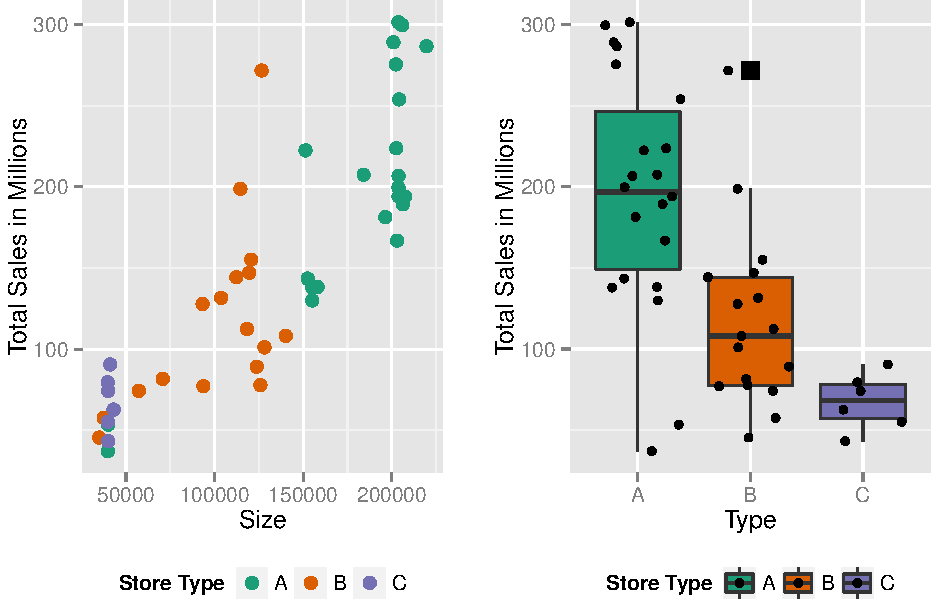
\includegraphics[width=400px]{PredictingWeeklySalesAtWalmart_files/figure-latex/storeTypeScatterBoxGrid-1}

\begin{Shaded}
\begin{Highlighting}[]
\NormalTok{## removing the plots from memory}
\KeywordTok{rm}\NormalTok{( scatterPlotStoreSize , boxplotStoreSize )}
\end{Highlighting}
\end{Shaded}

This plot indicates that there is a postie relationship between the size
of the store and total sales. Also Type `A' Stores are mostly larger
stores with bigger sales and Type `C' Stores are small with lower sales.

\begin{Shaded}
\begin{Highlighting}[]
\NormalTok{## calculating the summary statistics for each Type}
\NormalTok{tabledTypeWiseSummaryStatistics <-}\StringTok{ }
\StringTok{  }\KeywordTok{tapply}\NormalTok{(stores$TotalSalesInMillion , stores$Type , summary)}

\NormalTok{## Changing the Labels of the tabled Summary Statistics for printing}
\KeywordTok{attributes}\NormalTok{(tabledTypeWiseSummaryStatistics)$dimnames[[}\DecValTok{1}\NormalTok{]] <-}\StringTok{ }
\StringTok{  }\KeywordTok{c}\NormalTok{( }
    \StringTok{"Type A Store Summary Statistics"} \NormalTok{, }
    \StringTok{"Type B Store Summary Statistics"} \NormalTok{, }
    \StringTok{"Type C Store Summary Statistics"} \NormalTok{)}

\NormalTok{## Printing Summary Statistics for each Type of Store (based on Total Sales)}
\NormalTok{tabledTypeWiseSummaryStatistics}
\end{Highlighting}
\end{Shaded}

\begin{verbatim}
## $`Type A Store Summary Statistics`
##    Min. 1st Qu.  Median    Mean 3rd Qu.    Max. 
##   37.16  149.30  196.80  196.90  246.30  301.40 
## 
## $`Type B Store Summary Statistics`
##    Min. 1st Qu.  Median    Mean 3rd Qu.    Max. 
##   45.48   77.79  108.10  117.70  144.30  271.60 
## 
## $`Type C Store Summary Statistics`
##    Min. 1st Qu.  Median    Mean 3rd Qu.    Max. 
##   43.29   57.05   68.46   67.58   78.23   90.57
\end{verbatim}

\begin{Shaded}
\begin{Highlighting}[]
\NormalTok{## Removing table - not needed for further calculations}
\KeywordTok{rm}\NormalTok{( tabledTypeWiseSummaryStatistics )}
\end{Highlighting}
\end{Shaded}

From the graph, we can notice a Type B Outlier. A value is considered an
outlier when it's more than 3 Standard Deviations from the mean.

From this we can hypothesize that the Type of store could be an
important predictor of Weekly\_Sales.

\subsubsection{3.3.3 Total Sales Per Week - Time
Series}\label{total-sales-per-week---time-series}

We discuss here the effect holidays have on Total Sales of 45 Stores.

\begin{Shaded}
\begin{Highlighting}[]
\NormalTok{## Running tapply with sum to find the total sales per week}
\NormalTok{totalSalesPerWeek <-}\StringTok{ }
\StringTok{  }\KeywordTok{tapply}\NormalTok{( }
    \NormalTok{trainStoresFeaturesMerge$Weekly_Sales , }
    \NormalTok{trainStoresFeaturesMerge$Date , }
    \DataTypeTok{FUN =} \NormalTok{sum )}
\NormalTok{## Converting table to Data Frame}
\NormalTok{totalSalesPerWeekDataFrame <-}\StringTok{ }\KeywordTok{as.data.frame}\NormalTok{( totalSalesPerWeek )}
\NormalTok{## Converting date from String-Factor to Date Type}
\NormalTok{totalSalesPerWeekDataFrame$Date <-}\StringTok{ }
\StringTok{  }\KeywordTok{as.Date}\NormalTok{( }\KeywordTok{rownames}\NormalTok{(totalSalesPerWeekDataFrame ) )}
\NormalTok{## Renaming the Column to "TotalSales"}
\KeywordTok{colnames}\NormalTok{(totalSalesPerWeekDataFrame)[}\DecValTok{1}\NormalTok{] <-}\StringTok{ "TotalSales"}
\NormalTok{## Calculating the Total sales in Millions}
\NormalTok{totalSalesPerWeekDataFrame$TotalSalesInMillion =}\StringTok{ }
\StringTok{  }\NormalTok{totalSalesPerWeekDataFrame$TotalSales/}\DecValTok{1000000}
\end{Highlighting}
\end{Shaded}

\begin{Shaded}
\begin{Highlighting}[]
\NormalTok{## function to handle lag}
\NormalTok{## Since the in-built function in R to handle LAG is not working}
\NormalTok{## x - vector that needs to be lagged}
\NormalTok{## k - is the no of lags that need to be returned as a vector }
\NormalTok{##   - may be positive or negative}
\NormalTok{##   - it returns 0 instead of NA for the missing values}
\NormalTok{## returns a vector contained the lagged data with padded 0s for missing data}
\NormalTok{lagpad <-}\StringTok{ }\NormalTok{function(x, k) \{}
  \NormalTok{if( k >}\StringTok{ }\DecValTok{0} \NormalTok{) \{}
    \CommentTok{# It should actually be NA in the rep function}
    \KeywordTok{c}\NormalTok{(}\KeywordTok{rep}\NormalTok{(}\DecValTok{0}\NormalTok{, k), x)[}\DecValTok{1} \NormalTok{:}\StringTok{ }\KeywordTok{length}\NormalTok{(x)] }
  \NormalTok{\} else \{}
    \CommentTok{# It should actually be NA in the rep function}
    \KeywordTok{c}\NormalTok{(x[ (}\KeywordTok{abs}\NormalTok{(k)+}\DecValTok{1}\NormalTok{) :}\StringTok{ }\KeywordTok{length}\NormalTok{(x)] , }\KeywordTok{rep}\NormalTok{(}\DecValTok{0}\NormalTok{, }\KeywordTok{abs}\NormalTok{(k) ) )  }
  \NormalTok{\}}
\NormalTok{\}}
\end{Highlighting}
\end{Shaded}

\begin{Shaded}
\begin{Highlighting}[]
\NormalTok{## Getting the holiday List}
\NormalTok{## Extracting the Holiday List}
\NormalTok{holidayDateTable <-}\StringTok{ }
\StringTok{  }\KeywordTok{table}\NormalTok{(trainStoresFeaturesMerge$Date , trainStoresFeaturesMerge$IsHoliday)}
\NormalTok{## Converting from Table to Data Frame}
\NormalTok{holidayDateTableDataFrame <-}\StringTok{ }\KeywordTok{as.data.frame}\NormalTok{( holidayDateTable)}
\NormalTok{## Extracting the Holidays}
\NormalTok{holidayDateTableDataFrame <-}\StringTok{ }
\StringTok{  }\KeywordTok{subset}\NormalTok{( holidayDateTableDataFrame,holidayDateTableDataFrame$Var2==T)}
\NormalTok{## Marking the Holdiays in the dataset}
\NormalTok{holidayDateTableDataFrame$IsHoliday <-}\StringTok{ }
\StringTok{  }\KeywordTok{ifelse}\NormalTok{( holidayDateTableDataFrame$Freq >}\DecValTok{0} \NormalTok{, }\DecValTok{1} \NormalTok{, }\DecValTok{0} \NormalTok{)}
\NormalTok{## Converting Date from String-Factor to Date Type}
\NormalTok{holidayDateTableDataFrame$Date <-}\StringTok{ }\KeywordTok{as.Date}\NormalTok{( holidayDateTableDataFrame$Var1 )}
\CommentTok{# creating the holiday season - before and after the holiday week - 2 weeks}
\NormalTok{holidayDateTableDataFrame$Week1BeforeHoliday <-}\StringTok{ }
\StringTok{  }\KeywordTok{lagpad}\NormalTok{(holidayDateTableDataFrame$IsHoliday , -}\DecValTok{1}\NormalTok{)}
\NormalTok{holidayDateTableDataFrame$Week2BeforeHoliday <-}\StringTok{ }
\StringTok{  }\KeywordTok{lagpad}\NormalTok{(holidayDateTableDataFrame$IsHoliday , -}\DecValTok{2}\NormalTok{)}
\NormalTok{holidayDateTableDataFrame$Week1AfterHoliday <-}\StringTok{ }
\StringTok{  }\KeywordTok{lagpad}\NormalTok{(holidayDateTableDataFrame$IsHoliday , }\DecValTok{1}\NormalTok{)}
\NormalTok{holidayDateTableDataFrame$Week2AfterHoliday <-}\StringTok{ }
\StringTok{  }\KeywordTok{lagpad}\NormalTok{(holidayDateTableDataFrame$IsHoliday , }\DecValTok{2}\NormalTok{)}
\NormalTok{## Creating an ordered Holiday Season Type}
\NormalTok{holidayDateTableDataFrame$HolidaySeasonType =}\StringTok{ }
\StringTok{  }\KeywordTok{ifelse}\NormalTok{( holidayDateTableDataFrame$Week1BeforeHoliday ==}\StringTok{ }\DecValTok{1} \NormalTok{, }
          \StringTok{"1 Week Before"} \NormalTok{,}
          \KeywordTok{ifelse}\NormalTok{( }
            \NormalTok{holidayDateTableDataFrame$Week2BeforeHoliday ==}\StringTok{ }\DecValTok{1} \NormalTok{, }
            \StringTok{"2 Weeks Before"} \NormalTok{,}
                  \KeywordTok{ifelse}\NormalTok{( }
                    \NormalTok{holidayDateTableDataFrame$Week1AfterHoliday ==}\StringTok{ }\DecValTok{1} \NormalTok{, }
                    \StringTok{"1 Week After"} \NormalTok{,}
                          \KeywordTok{ifelse}\NormalTok{( }
                            \NormalTok{holidayDateTableDataFrame$Week2AfterHoliday ==}\StringTok{ }\DecValTok{1} \NormalTok{,}
                            \StringTok{"2 Weeks After"} \NormalTok{,}
                                  \KeywordTok{ifelse}\NormalTok{( }
                                    \NormalTok{holidayDateTableDataFrame$IsHoliday ==}\StringTok{ }\DecValTok{1} \NormalTok{, }
                                          \StringTok{"Holiday Week"} \NormalTok{, }\StringTok{"No Holiday"} \NormalTok{)))))}
\NormalTok{holidayDateTableDataFrame$HolidaySeasonType =}\StringTok{ }\KeywordTok{factor}\NormalTok{(}
  \NormalTok{holidayDateTableDataFrame$HolidaySeasonType , }
  \DataTypeTok{ordered=}\OtherTok{TRUE} \NormalTok{, }
  \DataTypeTok{levels=}\KeywordTok{c}\NormalTok{( }
    \StringTok{"No Holiday"} \NormalTok{,}
    \StringTok{"2 Weeks Before"} \NormalTok{,}
    \StringTok{"1 Week Before"} \NormalTok{,}
    \StringTok{"Holiday Week"} \NormalTok{,}
    \StringTok{"1 Week After"} \NormalTok{,}
    \StringTok{"2 Weeks After"}
    \NormalTok{)}
  \NormalTok{)}

\NormalTok{## Creating a variable to mark if it is a Holiday season - }
\NormalTok{## that is 2 weeks before + holdiay week + 2 weeks after}
\NormalTok{holidayDateTableDataFrame$IsHolidaySeason <-}\StringTok{ }
\StringTok{  }\NormalTok{holidayDateTableDataFrame$IsHoliday +}
\StringTok{  }\NormalTok{holidayDateTableDataFrame$Week1BeforeHoliday *}\StringTok{ }\NormalTok{.}\DecValTok{6} \NormalTok{+}
\StringTok{  }\NormalTok{holidayDateTableDataFrame$Week2BeforeHoliday *.}\DecValTok{2}   \NormalTok{+}
\StringTok{  }\NormalTok{holidayDateTableDataFrame$Week1AfterHoliday *}\StringTok{ }\NormalTok{.}\DecValTok{6} \NormalTok{+}
\StringTok{  }\NormalTok{holidayDateTableDataFrame$Week2AfterHoliday *.}\DecValTok{2}

\NormalTok{## Removing unneccesary Columns}
\NormalTok{holidayDateTableDataFrame$Var1 =}\StringTok{ }
\StringTok{  }\NormalTok{holidayDateTableDataFrame$Var2 =}\StringTok{ }
\StringTok{  }\NormalTok{holidayDateTableDataFrame$Freq =}\StringTok{ }\OtherTok{NULL}
\NormalTok{## Clearing Memory - removing intermediate Tables }
\KeywordTok{rm}\NormalTok{( holidayDateTable , totalSalesPerWeek )}
\end{Highlighting}
\end{Shaded}

\begin{Shaded}
\begin{Highlighting}[]
\NormalTok{## Mering the sales per week and holiday list }
\NormalTok{totalSalesPerWeekDataFrame <-}\StringTok{ }
\StringTok{  }\KeywordTok{merge}\NormalTok{( totalSalesPerWeekDataFrame, holidayDateTableDataFrame , }\DataTypeTok{by=}\DecValTok{2}\NormalTok{)}
\end{Highlighting}
\end{Shaded}

\begin{Shaded}
\begin{Highlighting}[]
\CommentTok{# Plotting Sales Per Week}
\KeywordTok{ggplot}\NormalTok{( totalSalesPerWeekDataFrame , }
        \KeywordTok{aes}\NormalTok{(}\DataTypeTok{x=}\NormalTok{Date , }\DataTypeTok{y=}\NormalTok{TotalSalesInMillion , }\DataTypeTok{color =} \NormalTok{HolidaySeasonType ) ) +}\StringTok{ }
\StringTok{  }\KeywordTok{geom_line}\NormalTok{( }\KeywordTok{aes}\NormalTok{(}\DataTypeTok{group=}\DecValTok{1}\NormalTok{) ) +}\StringTok{ }
\StringTok{  }\KeywordTok{geom_point}\NormalTok{(}\DataTypeTok{size =} \DecValTok{2}\NormalTok{) +}
\StringTok{  }\KeywordTok{scale_y_continuous}\NormalTok{(}\DataTypeTok{name=}\StringTok{"Total Sales in Millions"} \NormalTok{) +}
\StringTok{  }\KeywordTok{scale_color_brewer}\NormalTok{(}\DataTypeTok{palette=}\StringTok{"Dark2"} \NormalTok{, }\DataTypeTok{name =} \StringTok{"Season Type"}\NormalTok{)}
\end{Highlighting}
\end{Shaded}

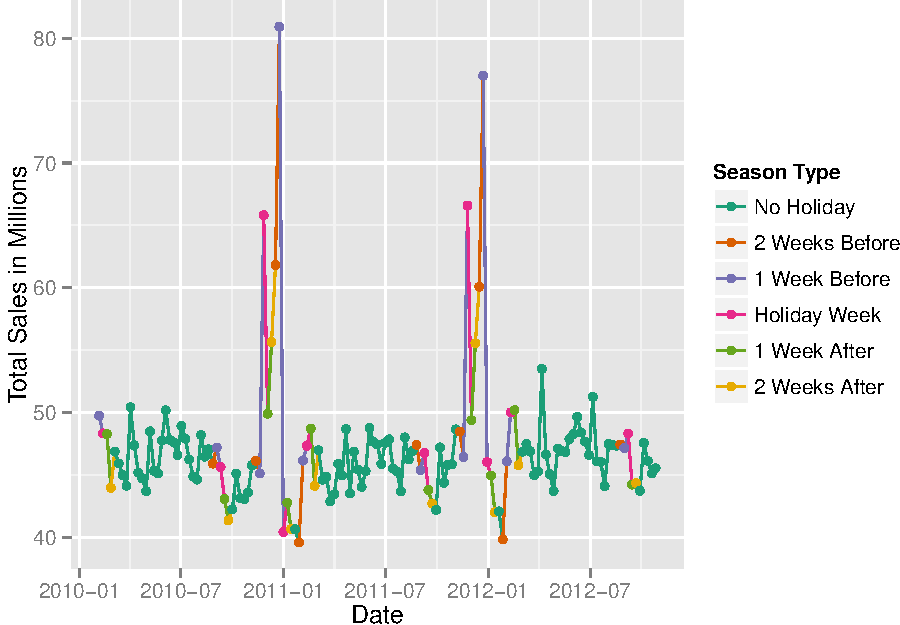
\includegraphics[width=400px]{PredictingWeeklySalesAtWalmart_files/figure-latex/plottingSalesPerWeek-1}

We can clearly see some trends here:

\begin{itemize}
\itemsep1pt\parskip0pt\parsep0pt
\item
  Sales go up a week before the holiday week
\item
  It is a repeating pattern - towards the end of the year, there is more
  sales - perhaps because of Thanksgiving and Christmas.
\item
  Average Total Sales per week is between 45-50 million Dollars (for 45
  stores in the dataset)
\item
  Perhaps the Data given incorrectly marks the Holiday Week for
  Christmas - it is marked as the dates 27, 28, 30 \& 31 across
  different years. But looking at the peak, the highest sales for
  Christmas is the week before - which is perhaps the more accurate
  holiday week
\item
  To be able to make better predictors, perhaps it would help to
  actually create separate factors for each of the holidays
\item
  It will be interesting to study the period between Aug 27, 2010 to Feb
  25, 2011. This section has all the holidays - starting with Labor Day,
  Thanksgiving, Christmas \& Super Bowl. Since the dataset will be
  smaller, we will perhaps understand the data better.
\end{itemize}

\begin{Shaded}
\begin{Highlighting}[]
\NormalTok{#####################################}
\CommentTok{# Creating separate holiday dummy variables}
\NormalTok{holidayDateTableDataFrame$IsHolidayDefined <-}\StringTok{ }
\StringTok{  }\KeywordTok{ifelse}\NormalTok{( }
    \NormalTok{holidayDateTableDataFrame$IsHoliday ==}\StringTok{ }\DecValTok{1} \NormalTok{&}\StringTok{ }
\StringTok{      }\KeywordTok{month}\NormalTok{( holidayDateTableDataFrame$Date ) ==}\StringTok{ }\DecValTok{2} \NormalTok{,}
          \DecValTok{2}\NormalTok{, }\KeywordTok{ifelse}\NormalTok{( }
            \NormalTok{holidayDateTableDataFrame$IsHoliday ==}\StringTok{ }\DecValTok{1} \NormalTok{&}\StringTok{ }
\StringTok{              }\KeywordTok{month}\NormalTok{( holidayDateTableDataFrame$Date ) ==}\StringTok{ }\DecValTok{9} \NormalTok{,}
                     \DecValTok{9} \NormalTok{, }\KeywordTok{ifelse}\NormalTok{( }
                       \NormalTok{holidayDateTableDataFrame$IsHoliday ==}\StringTok{ }\DecValTok{1} \NormalTok{&}\StringTok{ }
\StringTok{                         }\KeywordTok{month}\NormalTok{( holidayDateTableDataFrame$Date ) ==}\StringTok{ }\DecValTok{11} \NormalTok{,}
                                 \DecValTok{11} \NormalTok{, }\KeywordTok{ifelse}\NormalTok{( }
                                   \NormalTok{holidayDateTableDataFrame$IsHoliday ==}\StringTok{ }\DecValTok{1} \NormalTok{&}\StringTok{ }
\StringTok{                                     }\KeywordTok{month}\NormalTok{( }
                                       \NormalTok{holidayDateTableDataFrame$Date ) ==}\StringTok{ }\DecValTok{12} \NormalTok{,}
                                              \DecValTok{12} \NormalTok{, }\DecValTok{0} \NormalTok{) ) ) )}
\CommentTok{# creating the holiday season lag - before and after the holiday week - 2 weeks}
\NormalTok{holidayDateTableDataFrame$Week1BeforeHoliday <-}\StringTok{ }
\StringTok{  }\KeywordTok{lagpad}\NormalTok{(holidayDateTableDataFrame$IsHolidayDefined , -}\DecValTok{1}\NormalTok{)}
\NormalTok{holidayDateTableDataFrame$Week2BeforeHoliday <-}\StringTok{ }
\StringTok{  }\KeywordTok{lagpad}\NormalTok{(holidayDateTableDataFrame$IsHolidayDefined , -}\DecValTok{2}\NormalTok{)}
\NormalTok{holidayDateTableDataFrame$Week1AfterHoliday <-}\StringTok{ }
\StringTok{  }\KeywordTok{lagpad}\NormalTok{(holidayDateTableDataFrame$IsHolidayDefined , }\DecValTok{1}\NormalTok{)}
\NormalTok{holidayDateTableDataFrame$Week2AfterHoliday <-}\StringTok{ }
\StringTok{  }\KeywordTok{lagpad}\NormalTok{(holidayDateTableDataFrame$IsHolidayDefined , }\DecValTok{2}\NormalTok{)}

\NormalTok{## Creating a variable to hold the holiday type season id}
\NormalTok{holidayDateTableDataFrame$HolidaySeasonId <-}\StringTok{ }\KeywordTok{as.factor}\NormalTok{(}
  \NormalTok{holidayDateTableDataFrame$Week1BeforeHoliday +}\StringTok{ }
\StringTok{  }\NormalTok{holidayDateTableDataFrame$Week2BeforeHoliday +}
\StringTok{  }\NormalTok{holidayDateTableDataFrame$IsHolidayDefined +}
\StringTok{  }\NormalTok{holidayDateTableDataFrame$Week1AfterHoliday +}
\StringTok{  }\NormalTok{holidayDateTableDataFrame$Week2AfterHoliday )}


\NormalTok{## Creating an ordered Holiday Season Type for Super Bowl}
\NormalTok{holidayDateTableDataFrame$HolidaySeasonType <-}\StringTok{ }
\StringTok{  }\KeywordTok{ifelse}\NormalTok{( }
    \NormalTok{holidayDateTableDataFrame$Week1BeforeHoliday ==}\StringTok{ }\DecValTok{2} \NormalTok{, }
    \StringTok{"1 Week Before Super Bowl"} \NormalTok{,}
          \KeywordTok{ifelse}\NormalTok{( }
            \NormalTok{holidayDateTableDataFrame$Week2BeforeHoliday ==}\StringTok{ }\DecValTok{2} \NormalTok{, }
            \StringTok{"2 Weeks Before Super Bowl"} \NormalTok{,}
                  \KeywordTok{ifelse}\NormalTok{( }
                    \NormalTok{holidayDateTableDataFrame$Week1AfterHoliday ==}\StringTok{ }\DecValTok{2} \NormalTok{, }
                    \StringTok{"1 Week After Super Bowl"} \NormalTok{,}
                          \KeywordTok{ifelse}\NormalTok{( }
                            \NormalTok{holidayDateTableDataFrame$Week2AfterHoliday ==}\StringTok{ }\DecValTok{2} \NormalTok{,}
                            \StringTok{"2 Weeks After Super Bowl"} \NormalTok{,}
                                  \KeywordTok{ifelse}\NormalTok{( }
                                    \NormalTok{holidayDateTableDataFrame$IsHolidayDefined }
                                    \NormalTok{==}\StringTok{ }\DecValTok{2} \NormalTok{,}
                                    \StringTok{"Super Bowl"} \NormalTok{, }\StringTok{"No Holiday"} \NormalTok{)))))}

\NormalTok{## Creating an ordered Holiday Season Type for Labor Day}
\NormalTok{holidayDateTableDataFrame$HolidaySeasonType <-}\StringTok{ }
\StringTok{  }\KeywordTok{ifelse}\NormalTok{( }
    \NormalTok{holidayDateTableDataFrame$Week1BeforeHoliday ==}\StringTok{ }\DecValTok{9} \NormalTok{, }
    \StringTok{"1 Week Before Labor Day"} \NormalTok{,}
          \KeywordTok{ifelse}\NormalTok{( }
            \NormalTok{holidayDateTableDataFrame$Week2BeforeHoliday ==}\StringTok{ }\DecValTok{9} \NormalTok{, }
            \StringTok{"2 Weeks Before Labor Day"} \NormalTok{,}
                  \KeywordTok{ifelse}\NormalTok{( }
                    \NormalTok{holidayDateTableDataFrame$Week1AfterHoliday ==}\StringTok{ }\DecValTok{9} \NormalTok{, }
                    \StringTok{"1 Week After Labor Day"} \NormalTok{,}
                          \KeywordTok{ifelse}\NormalTok{( }
                            \NormalTok{holidayDateTableDataFrame$Week2AfterHoliday ==}\StringTok{ }\DecValTok{9} \NormalTok{,}
                            \StringTok{"2 Weeks After Labor Day"} \NormalTok{,}
                                  \KeywordTok{ifelse}\NormalTok{( }
                                    \NormalTok{holidayDateTableDataFrame$IsHolidayDefined }
                                    \NormalTok{==}\StringTok{ }\DecValTok{9} \NormalTok{, }\StringTok{"Labor Day"} \NormalTok{,}
                                    \NormalTok{holidayDateTableDataFrame$HolidaySeasonType }
                                    \NormalTok{) ) ) ) )}

\NormalTok{## Creating an ordered Holiday Season Type for Thanksgiving}
\NormalTok{holidayDateTableDataFrame$HolidaySeasonType <-}\StringTok{ }
\StringTok{  }\KeywordTok{ifelse}\NormalTok{( }
    \NormalTok{holidayDateTableDataFrame$Week1BeforeHoliday ==}\StringTok{ }\DecValTok{11} \NormalTok{, }
    \StringTok{"1 Week Before Thanksgiving"} \NormalTok{,}
          \KeywordTok{ifelse}\NormalTok{( }
            \NormalTok{holidayDateTableDataFrame$Week2BeforeHoliday ==}\StringTok{ }\DecValTok{11} \NormalTok{, }
            \StringTok{"2 Weeks Before Thanksgiving"} \NormalTok{,}
                  \KeywordTok{ifelse}\NormalTok{( }
                    \NormalTok{holidayDateTableDataFrame$Week1AfterHoliday ==}\StringTok{ }\DecValTok{11} \NormalTok{, }
                    \StringTok{"1 Week After Thanksgiving"} \NormalTok{,}
                          \KeywordTok{ifelse}\NormalTok{( }
                            \NormalTok{holidayDateTableDataFrame$Week2AfterHoliday ==}\StringTok{ }\DecValTok{11} \NormalTok{,}
                            \StringTok{"2 Weeks After Thanksgiving"} \NormalTok{,}
                                  \KeywordTok{ifelse}\NormalTok{( }
                                    \NormalTok{holidayDateTableDataFrame$IsHolidayDefined }
                                    \NormalTok{==}\StringTok{ }\DecValTok{11} \NormalTok{, }\StringTok{"Thanksgiving"} \NormalTok{,}
                                    \NormalTok{holidayDateTableDataFrame$HolidaySeasonType }
                                    \NormalTok{) ) ) ) )}

\NormalTok{## Creating an ordered Holiday Season Type for Christmas}
\NormalTok{holidayDateTableDataFrame$HolidaySeasonType <-}\StringTok{ }
\StringTok{  }\KeywordTok{ifelse}\NormalTok{( }
    \NormalTok{holidayDateTableDataFrame$Week1BeforeHoliday ==}\StringTok{ }\DecValTok{12} \NormalTok{, }
    \StringTok{"1 Week Before Christmas"} \NormalTok{,}
          \KeywordTok{ifelse}\NormalTok{( }
            \NormalTok{holidayDateTableDataFrame$Week2BeforeHoliday ==}\StringTok{ }\DecValTok{12} \NormalTok{, }
            \StringTok{"2 Weeks Before Christmas"} \NormalTok{,}
                  \KeywordTok{ifelse}\NormalTok{( }
                    \NormalTok{holidayDateTableDataFrame$Week1AfterHoliday ==}\StringTok{ }\DecValTok{12} \NormalTok{, }
                    \StringTok{"1 Week After Christmas"} \NormalTok{,}
                          \KeywordTok{ifelse}\NormalTok{( }
                            \NormalTok{holidayDateTableDataFrame$Week2AfterHoliday ==}\StringTok{ }\DecValTok{12} \NormalTok{, }
                            \StringTok{"2 Weeks After Christmas"} \NormalTok{,}
                                  \KeywordTok{ifelse}\NormalTok{( }
                                    \NormalTok{holidayDateTableDataFrame$IsHolidayDefined }
                                    \NormalTok{==}\StringTok{ }\DecValTok{12} \NormalTok{, }\StringTok{"Christmas"} \NormalTok{,}
                                    \NormalTok{holidayDateTableDataFrame$HolidaySeasonType }
                                    \NormalTok{) ) ) ) )}

\NormalTok{holidayDateTableDataFrame$HolidaySeasonType =}\StringTok{ }\KeywordTok{factor}\NormalTok{(}
  \NormalTok{holidayDateTableDataFrame$HolidaySeasonType , }
  \DataTypeTok{ordered=}\OtherTok{TRUE} \NormalTok{, }
  \DataTypeTok{levels=}\KeywordTok{c}\NormalTok{( }
    \StringTok{"No Holiday"} \NormalTok{,}
    \StringTok{"2 Weeks Before Super Bowl"} \NormalTok{,}
    \StringTok{"1 Week Before Super Bowl"} \NormalTok{,}
    \StringTok{"Super Bowl"} \NormalTok{,}
    \StringTok{"1 Week After Super Bowl"} \NormalTok{,}
    \StringTok{"2 Weeks After Super Bowl"} \NormalTok{,}
    \StringTok{"2 Weeks Before Labor Day"} \NormalTok{,}
    \StringTok{"1 Week Before Labor Day"} \NormalTok{,}
    \StringTok{"Labor Day"} \NormalTok{,}
    \StringTok{"1 Week After Labor Day"} \NormalTok{,}
    \StringTok{"2 Weeks After Labor Day"} \NormalTok{,}
    \StringTok{"2 Weeks Before Thanksgiving"} \NormalTok{,}
    \StringTok{"1 Week Before Thanksgiving"} \NormalTok{,}
    \StringTok{"Thanksgiving"} \NormalTok{,}
    \StringTok{"1 Week After Thanksgiving"} \NormalTok{,}
    \StringTok{"2 Weeks After Thanksgiving"} \NormalTok{,}
    \StringTok{"2 Weeks Before Christmas"} \NormalTok{,}
    \StringTok{"1 Week Before Christmas"} \NormalTok{,}
    \StringTok{"Christmas"} \NormalTok{,}
    \StringTok{"1 Week After Christmas"} \NormalTok{,}
    \StringTok{"2 Weeks After Christmas"}
  \NormalTok{)}
\NormalTok{)}
\end{Highlighting}
\end{Shaded}

\begin{Shaded}
\begin{Highlighting}[]
\NormalTok{## Mering the sales per week and holiday list }
\NormalTok{totalSalesPerWeekDataFrame$HolidaySeasonType <-}\StringTok{ }
\StringTok{  }\NormalTok{holidayDateTableDataFrame$HolidaySeasonType}
\NormalTok{## Merging the season Type with sales per week}
\NormalTok{totalSalesPerWeekDataFrame$HolidaySeasonId <-}\StringTok{ }
\StringTok{  }\NormalTok{holidayDateTableDataFrame$HolidaySeasonId}
\end{Highlighting}
\end{Shaded}

\begin{Shaded}
\begin{Highlighting}[]
\NormalTok{## Subsetting only the holidays}
\NormalTok{totalSalesPerWeekDataFrameDuringHolidays <-}\StringTok{ }
\StringTok{  }\KeywordTok{subset}\NormalTok{( totalSalesPerWeekDataFrame , }
          \NormalTok{totalSalesPerWeekDataFrame$Date >=}\StringTok{ '2010-08-27'} \NormalTok{&}\StringTok{ }
\StringTok{            }\NormalTok{totalSalesPerWeekDataFrame$Date <=}\StringTok{ '2011-02-25'} \NormalTok{)}
\end{Highlighting}
\end{Shaded}

\begin{Shaded}
\begin{Highlighting}[]
\NormalTok{## Plotting the subset of totalSalesPerWeekDataFrame}
\KeywordTok{ggplot}\NormalTok{( totalSalesPerWeekDataFrameDuringHolidays , }
        \KeywordTok{aes}\NormalTok{(}\DataTypeTok{x=}\NormalTok{Date , }\DataTypeTok{y=}\NormalTok{TotalSalesInMillion , }
            \DataTypeTok{color =} \NormalTok{HolidaySeasonId ) ) +}\StringTok{ }
\StringTok{  }\KeywordTok{geom_line}\NormalTok{( }\KeywordTok{aes}\NormalTok{(}\DataTypeTok{group=}\DecValTok{1}\NormalTok{) ) +}\StringTok{ }
\StringTok{  }\KeywordTok{geom_point}\NormalTok{(}\DataTypeTok{size =} \DecValTok{2}\NormalTok{) +}
\StringTok{  }\KeywordTok{scale_y_continuous}\NormalTok{(}\DataTypeTok{name=}\StringTok{"Total Sales in Millions"} \NormalTok{)  +}
\StringTok{  }\KeywordTok{scale_color_brewer}\NormalTok{(}
    \DataTypeTok{palette=}\StringTok{"Dark2"} \NormalTok{, }
    \DataTypeTok{name =} \StringTok{"Holiday Season"} \NormalTok{,}
    \DataTypeTok{labels =} \KeywordTok{c}\NormalTok{( }
      \StringTok{"No Holiday"} \NormalTok{, }
      \StringTok{"Super Bowl"} \NormalTok{,}
      \StringTok{"Labor Day"} \NormalTok{, }
      \StringTok{"Thanksgiving"} \NormalTok{,}
      \StringTok{"Christmas"}
      \NormalTok{)}
    \NormalTok{) }
\end{Highlighting}
\end{Shaded}

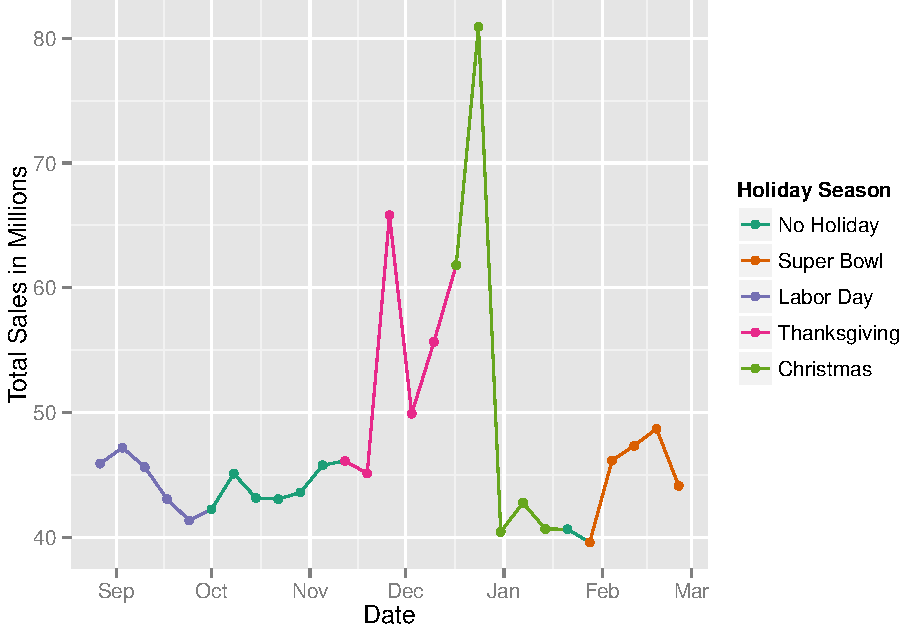
\includegraphics[width=400px]{PredictingWeeklySalesAtWalmart_files/figure-latex/plottingSubsetOfHolidays-1}

\begin{Shaded}
\begin{Highlighting}[]
\NormalTok{## removing the following columns because it may cause }
\NormalTok{## multi-collinearity issues once merged with the main data and}
\NormalTok{## building a model with that}
\NormalTok{holidayDateTableDataFrame$Week1BeforeHoliday =}\StringTok{ }\OtherTok{NULL}
\NormalTok{holidayDateTableDataFrame$Week2BeforeHoliday =}\StringTok{ }\OtherTok{NULL}
\NormalTok{holidayDateTableDataFrame$Week1AfterHoliday =}\StringTok{ }\OtherTok{NULL}
\NormalTok{holidayDateTableDataFrame$Week2AfterHoliday =}\StringTok{ }\OtherTok{NULL}
\NormalTok{holidayDateTableDataFrame$IsHoliday =}\StringTok{ }\OtherTok{NULL}
\NormalTok{holidayDateTableDataFrame$IsHolidayDefined =}\StringTok{ }\OtherTok{NULL}
\NormalTok{## freeing memory}
\KeywordTok{rm}\NormalTok{( totalSalesPerWeekDataFrame , totalSalesPerWeekDataFrameDuringHolidays )}
\end{Highlighting}
\end{Shaded}

\subsubsection{3.3.4 Store-Department-wise Sales per Week - Time
Series}\label{store-department-wise-sales-per-week---time-series}

To see a representation of the granularity of the data, we would like to
plot all the data points of Weekly Sales vs Time (Week)

\begin{Shaded}
\begin{Highlighting}[]
\NormalTok{## plotting all the Weekly Sales figures - colored by Dept}
\KeywordTok{ggplot}\NormalTok{(trainStoresFeaturesMerge , }
       \KeywordTok{aes}\NormalTok{(}\DataTypeTok{x=}\NormalTok{Date , }\DataTypeTok{y =} \NormalTok{Weekly_Sales , }\DataTypeTok{color =} \NormalTok{Dept ) ) +}
\StringTok{  }\KeywordTok{geom_point}\NormalTok{() +}
\StringTok{  }\KeywordTok{scale_y_continuous}\NormalTok{(}\DataTypeTok{name=}\StringTok{"Weekly Sales"} \NormalTok{)}
\end{Highlighting}
\end{Shaded}

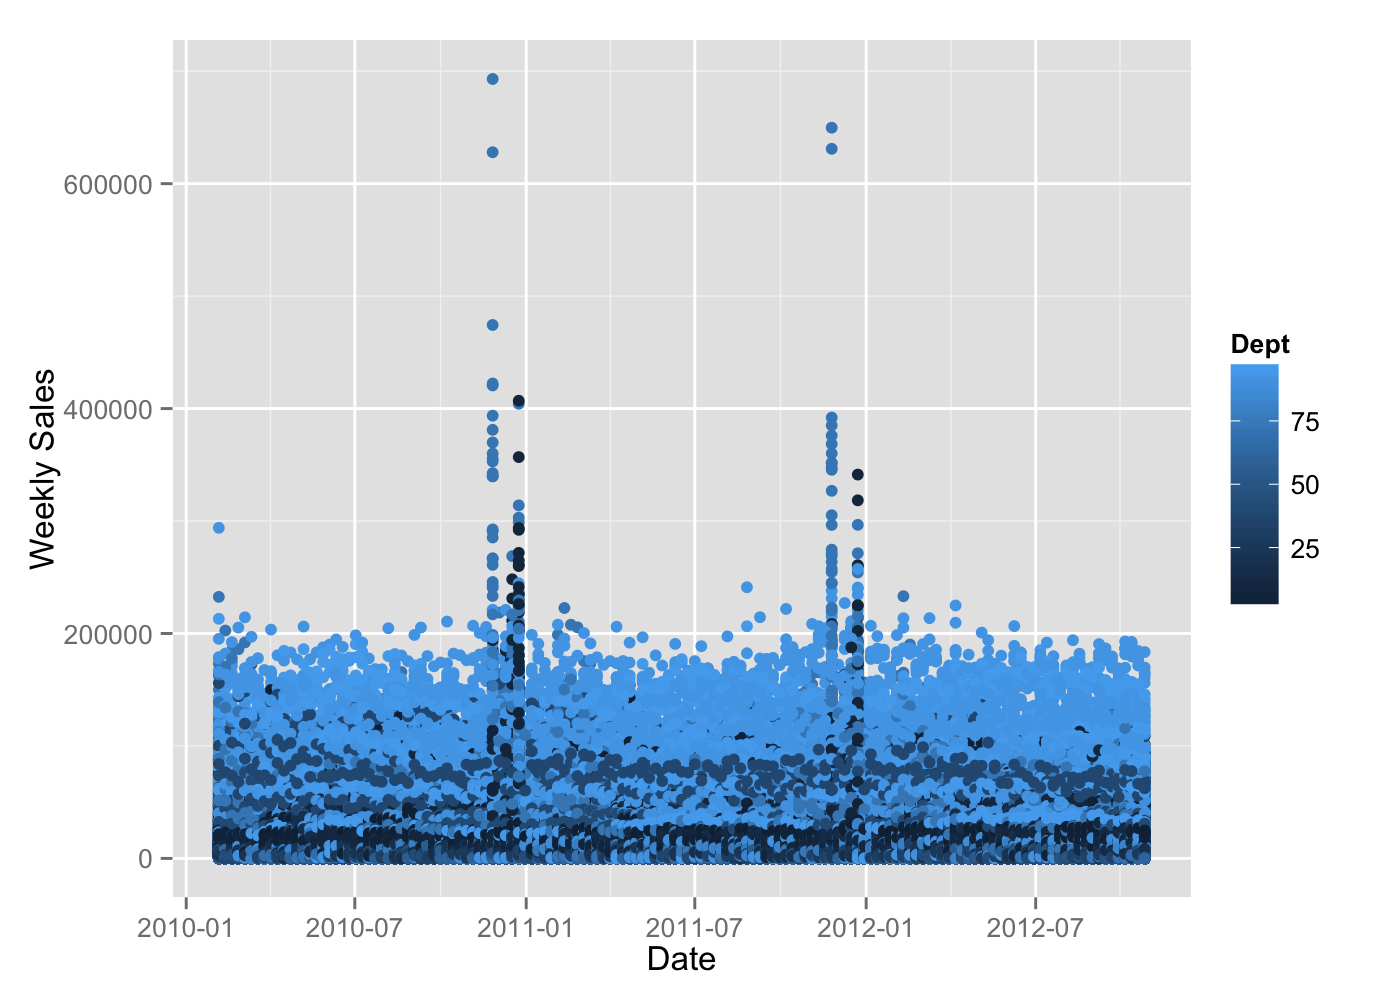
\includegraphics[width=400px]{PredictingWeeklySalesAtWalmart_files/figure-latex/allPoint-1}

While it is not easy to make sense of a graph with more than 400
thousand data points, here are some salient features that stand out:

\begin{itemize}
\itemsep1pt\parskip0pt\parsep0pt
\item
  Departments with the higher numbers (Dept\textgreater{}=75) have
  higher sales figures than the lower numbered departments (Dept
  \textless{}=25)
\item
  During Christmas we see a spike in a lower numbered department's sale
\item
  We see a repeating annual pattern. Possibly indicating that Week
  Numbers (eg: 50th week of the year) may be an important predictor
  variable
\end{itemize}

\begin{Shaded}
\begin{Highlighting}[]
\NormalTok{## Function to calculate Week}
\NormalTok{## date - the date for which the Week Number should be calculated}
\NormalTok{## returns week Number}
\NormalTok{weekNumber <-}\StringTok{ }\NormalTok{function( date ) \{}
  \NormalTok{d1 <-}\StringTok{ }\KeywordTok{as.Date}\NormalTok{( }\KeywordTok{paste0}\NormalTok{( }\KeywordTok{year}\NormalTok{(date) , }\StringTok{"-01-01"} \NormalTok{) )}
  \KeywordTok{as.integer}\NormalTok{((date-d1)/}\DecValTok{7}\NormalTok{)+}\DecValTok{1}
\NormalTok{\}}
\end{Highlighting}
\end{Shaded}

\begin{Shaded}
\begin{Highlighting}[]
\NormalTok{## Adding the Week Number to the holidayDateTableDataFrame}
\NormalTok{holidayDateTableDataFrame$WeekNumber <-}\StringTok{ }\KeywordTok{weekNumber}\NormalTok{( holidayDateTableDataFrame$Date )}
\NormalTok{## Adding Month to holidayDateTableDataFrame}
\NormalTok{holidayDateTableDataFrame$Month <-}\StringTok{ }\KeywordTok{month}\NormalTok{( holidayDateTableDataFrame$Date )}
\end{Highlighting}
\end{Shaded}

We have created Week and month numbers to influence the regression model
we will develop in Section 5.

\begin{Shaded}
\begin{Highlighting}[]
\NormalTok{## Merging holidayDateTableDataFrame with trainStoresFeaturesMerge}
\NormalTok{trainStoresFeaturesMerge <-}\StringTok{ }
\StringTok{  }\KeywordTok{merge}\NormalTok{( trainStoresFeaturesMerge , holidayDateTableDataFrame , }\DataTypeTok{by =} \StringTok{"Date"} \NormalTok{)}
\NormalTok{## removing holidayDateTableDataFrame from memory}
\KeywordTok{rm}\NormalTok{( holidayDateTableDataFrame )}
\end{Highlighting}
\end{Shaded}

\pagebreak

\section{4. Stage 2: Formal Statistical
Inferences}\label{stage-2-formal-statistical-inferences}

\subsection{4.1 On Average, Do Holiday Weeks Spike Sales
Up?}\label{on-average-do-holiday-weeks-spike-sales-up}

We would like to investigate if the sales figures are statistically
higher during holiday weeks. We have seen earlier that visually it does
appear that sales spike up during Thanksgiving and Christmas. We would
like to statistically verify this.

\subsubsection{4.1.1 The Hypotheses}\label{the-hypotheses}

Let us state our Hypotheses:

\begin{itemize}
\itemsep1pt\parskip0pt\parsep0pt
\item
  Null Hypothesis (H\textsubscript{0}) : On average, there is no
  difference in weekly sales figures during holiday weeks. In other
  words, there is no statisically significant difference between
  Weekly\_Sales numbers between holiday weeks and non-holiday weeks
\item
  Alternate Hypothesis (H\textsubscript{A}): Our alternate hypothesis is
  that there is a statistically significant higher sales figure during
  holiday weeks (one-sided test)
\end{itemize}

Mathematically, the hypothese are expressed below:

\begin{itemize}
\itemsep1pt\parskip0pt\parsep0pt
\item
  H\textsubscript{0}: μ\textsubscript{diff} = 0
\item
  H\textsubscript{A}: μ\textsubscript{diff} \textgreater{} 0
\end{itemize}

\subsubsection{4.1.2 The Data}\label{the-data}

We need to separate the datasets into Holiday and Non-holiday weeks and
then calculate the point estimate.

\begin{Shaded}
\begin{Highlighting}[]
\NormalTok{## Creating the datasets for Holiday and NotHoliday}
\NormalTok{Hyp_NotHoliday <-}\StringTok{ }\KeywordTok{subset}\NormalTok{( trainStoresFeaturesMerge , IsHoliday ==}\StringTok{ }\OtherTok{FALSE} \NormalTok{);}
\NormalTok{Hyp_Holiday <-}\StringTok{ }\KeywordTok{subset}\NormalTok{( trainStoresFeaturesMerge , IsHoliday ==}\StringTok{ }\OtherTok{TRUE} \NormalTok{);}

\NormalTok{## Getting the Number of rows in each dataset}
\KeywordTok{nrow}\NormalTok{( Hyp_NotHoliday )}
\end{Highlighting}
\end{Shaded}

\begin{verbatim}
## [1] 390652
\end{verbatim}

\begin{Shaded}
\begin{Highlighting}[]
\KeywordTok{nrow}\NormalTok{( Hyp_Holiday )}
\end{Highlighting}
\end{Shaded}

\begin{verbatim}
## [1] 29560
\end{verbatim}

\subsubsection{4.1.3 Central Limit Theorm: Checking the Conditions for
Hypothesis Testing for Paired
Data}\label{central-limit-theorm-checking-the-conditions-for-hypothesis-testing-for-paired-data}

The conditions for hypothesis testing:

\begin{itemize}
\itemsep1pt\parskip0pt\parsep0pt
\item
  Independence: Sampled observations must be independent. Random sample
  must be collected and if it is without replacement then the sample
  size must be less than 10\% of the Population
\item
  Sample Size / Skew: The no of elements must be more than 30.
\end{itemize}

We select a size of 2500 which is less than 10\% of Hyp\_Holiday.

\begin{Shaded}
\begin{Highlighting}[]
\NormalTok{## Number of sample elements to collect from population }
\NormalTok{## should be <10% of holiday Week Population}
\NormalTok{ndiff <-}\StringTok{ }\DecValTok{2500}
\NormalTok{## Seeding to ensure the randomness can be repeated}
\KeywordTok{set.seed}\NormalTok{(}\DecValTok{1101}\NormalTok{)}
\NormalTok{## Getting a sample of elements (ndiff) (<10% of Holiday Weeks)}
\NormalTok{Holiday_Sample <-}\StringTok{ }\KeywordTok{sample}\NormalTok{( Hyp_Holiday$Log_Weekly_Sales , ndiff )}
\KeywordTok{head}\NormalTok{(Holiday_Sample)}
\end{Highlighting}
\end{Shaded}

\begin{verbatim}
## [1]  9.917754  9.458827  8.332939  4.249637  9.247995 11.524153
\end{verbatim}

\begin{Shaded}
\begin{Highlighting}[]
\NormalTok{NotHoliday_Sample <-}\StringTok{ }\KeywordTok{sample}\NormalTok{( Hyp_NotHoliday$Log_Weekly_Sales , ndiff )}
\KeywordTok{head}\NormalTok{(NotHoliday_Sample)}
\end{Highlighting}
\end{Shaded}

\begin{verbatim}
## [1]  9.769958  7.077498  8.362108 10.209713  8.742134  5.934894
\end{verbatim}

\begin{Shaded}
\begin{Highlighting}[]
\NormalTok{## combining both the sample into one x-Axis Variable}
\NormalTok{xVar <-}\StringTok{ }\KeywordTok{c}\NormalTok{(NotHoliday_Sample , Holiday_Sample )}
\NormalTok{## Creating the color Variable}
\NormalTok{colorVar <-}\StringTok{ }\KeywordTok{as.factor}\NormalTok{(}\KeywordTok{c}\NormalTok{(}\KeywordTok{rep}\NormalTok{(}\DecValTok{1}\NormalTok{, ndiff), }\KeywordTok{rep}\NormalTok{(}\DecValTok{2}\NormalTok{, ndiff ) ) )}
\NormalTok{## creating the dataframe}
\NormalTok{sampleDensityDf <-}\StringTok{ }\KeywordTok{data.frame}\NormalTok{( xVar ,  colorVar )}
\NormalTok{## the density plot showing the }
\NormalTok{## Not Holiday and Holiday values of Log(Weekly_Sales)}
\NormalTok{plottingDensity <-}\StringTok{ }\KeywordTok{ggplot}\NormalTok{( sampleDensityDf , }\KeywordTok{aes}\NormalTok{(}\DataTypeTok{x =} \NormalTok{xVar, }\DataTypeTok{fill =} \NormalTok{colorVar) ) +}\StringTok{ }
\StringTok{  }\KeywordTok{geom_density}\NormalTok{( }\DataTypeTok{alpha =} \NormalTok{.}\DecValTok{2} \NormalTok{) +}
\StringTok{  }\KeywordTok{scale_x_continuous}\NormalTok{( }\StringTok{"log(Weekly_Sales)"} \NormalTok{) +}
\StringTok{  }\KeywordTok{scale_fill_discrete}\NormalTok{( }
    \DataTypeTok{name =} \StringTok{"Sample"} \NormalTok{, }\DataTypeTok{labels=}\KeywordTok{c}\NormalTok{( }\StringTok{"Not Holiday"}\NormalTok{, }\StringTok{"Holiday"} \NormalTok{) ) +}
\StringTok{  }\KeywordTok{scale_y_continuous}\NormalTok{( }\StringTok{"Density"} \NormalTok{) +}
\StringTok{  }\KeywordTok{theme}\NormalTok{( }\DataTypeTok{legend.position =} \StringTok{"bottom"} \NormalTok{)}
\NormalTok{## box plot to show the Density Distribution}
\NormalTok{boxPlotDensity <-}\StringTok{ }\KeywordTok{ggplot}\NormalTok{( sampleDensityDf , }\KeywordTok{aes}\NormalTok{( colorVar , xVar ) ) +}\StringTok{ }
\StringTok{  }\KeywordTok{geom_boxplot}\NormalTok{( }\KeywordTok{aes}\NormalTok{( }\DataTypeTok{fill =} \NormalTok{colorVar ) ) +}\StringTok{ }
\StringTok{  }\KeywordTok{scale_y_continuous}\NormalTok{( }\StringTok{"log(Weekly_Sales)"} \NormalTok{) +}
\StringTok{  }\KeywordTok{scale_fill_discrete}\NormalTok{( }
    \DataTypeTok{name =} \StringTok{"Sample"} \NormalTok{, }\DataTypeTok{labels=}\KeywordTok{c}\NormalTok{( }\StringTok{"Not Holiday"}\NormalTok{, }\StringTok{"Holiday"} \NormalTok{) ) +}
\StringTok{  }\KeywordTok{scale_x_discrete}\NormalTok{( }\StringTok{"Sample"} \NormalTok{, }\DataTypeTok{labels=}\KeywordTok{c}\NormalTok{( }\StringTok{"Not Holiday"}\NormalTok{, }\StringTok{"Holiday"} \NormalTok{)  ) +}
\StringTok{  }\KeywordTok{theme}\NormalTok{( }\DataTypeTok{legend.position =} \StringTok{"bottom"} \NormalTok{)}
\NormalTok{## arranging the plots next to each other}
\KeywordTok{grid.arrange}\NormalTok{( plottingDensity , boxPlotDensity , }\DataTypeTok{nrow =} \DecValTok{1} \NormalTok{)}
\end{Highlighting}
\end{Shaded}

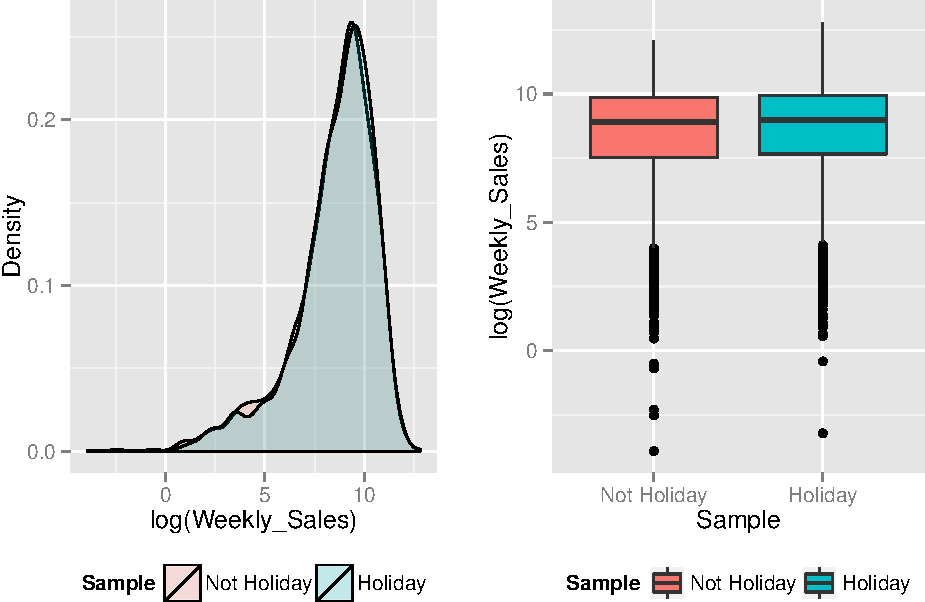
\includegraphics[width=400px]{PredictingWeeklySalesAtWalmart_files/figure-latex/visualizingTheSamplesCollected-1}

\begin{Shaded}
\begin{Highlighting}[]
\NormalTok{## removing plots from memory}
\KeywordTok{rm}\NormalTok{( xVar , colorVar , sampleDensityDf , plottingDensity , }
    \NormalTok{boxPlotDensity, Hyp_Holiday , Hyp_NotHoliday)}
\end{Highlighting}
\end{Shaded}

\subsubsection{4.1.4 Calculating the Test
Statistic}\label{calculating-the-test-statistic}

\begin{Shaded}
\begin{Highlighting}[]
\NormalTok{## Calculating the Difference}
\NormalTok{Diff_Log_Weekly_Sales =}\StringTok{ }\NormalTok{Holiday_Sample -}\StringTok{ }\NormalTok{NotHoliday_Sample}
\NormalTok{## Printing Top 5 values of diff}
\KeywordTok{head}\NormalTok{(Diff_Log_Weekly_Sales)}
\end{Highlighting}
\end{Shaded}

\begin{verbatim}
## [1]  0.14779642  2.38132920 -0.02916917 -5.96007556  0.50586191  5.58925841
\end{verbatim}

\begin{Shaded}
\begin{Highlighting}[]
\NormalTok{## Calculating the Test Statistic}
\NormalTok{xBar <-}\StringTok{ }\KeywordTok{mean}\NormalTok{(Diff_Log_Weekly_Sales)}
\NormalTok{xBar}
\end{Highlighting}
\end{Shaded}

\begin{verbatim}
## [1] 0.1026465
\end{verbatim}

\begin{Shaded}
\begin{Highlighting}[]
\NormalTok{## Calculating the Test Statistic}
\NormalTok{zScore <-}\StringTok{ }\NormalTok{xBar /}\StringTok{ }\KeywordTok{standardError}\NormalTok{(Diff_Log_Weekly_Sales)}
\NormalTok{zScore}
\end{Highlighting}
\end{Shaded}

\begin{verbatim}
## [1] 1.759381
\end{verbatim}

\begin{Shaded}
\begin{Highlighting}[]
\NormalTok{## Calculating p-value}
\NormalTok{## 1-pnorm() because we are doing a one-sided test - greater than}
\NormalTok{pValue <-}\StringTok{ }\DecValTok{1}\NormalTok{-}\KeywordTok{pnorm}\NormalTok{( zScore ) }
\NormalTok{pValue}
\end{Highlighting}
\end{Shaded}

\begin{verbatim}
## [1] 0.03925638
\end{verbatim}

\begin{Shaded}
\begin{Highlighting}[]
\NormalTok{## removing variables not needed anymore}
\KeywordTok{rm}\NormalTok{( pValue , zScore , xBar , Diff_Log_Weekly_Sales , Holiday_Sample , }
    \NormalTok{NotHoliday_Sample , ndiff )}
\end{Highlighting}
\end{Shaded}

\subsubsection{4.1.5 Decision: Alternate Hypothesis (H\textsubscript{A})
is Rejected}\label{decision-alternate-hypothesis-ha-is-rejected}

The \textbf{Null Hypothesis (H\textsubscript{0})} is NOT rejected
because the pValue is greater than the significance value of 0.05.

This imples that the Alternate Hypothesis (H\textsubscript{A}) is
rejected. Holiday weeks do not cause sales to spike up.

\subsubsection{4.1.6 Real World
Application}\label{real-world-application}

However, in graphs drawn in section 3.3.3 we were presented with another
reality. We saw the spike in sales during holiday season - Thanksgiving
and Christmas. One will recognize on close examination of the graphs
that most of the sales spike happened 1 week before the holiday week.
Sales during the holiday week was mostly on the decline from the high
sales peak from the week before.

Therefore, statistically, Holiday Week Sales are not very different from
that of non-holiday week sales. However, if we consider Holiday Season
sales, it may tell a different story. This will form the basis of our
next Hypothesis test - on average do Thanksgiving and Christmas
contribute to spike in sales?

\pagebreak

\subsection{4.2 On Average, Do Thanksgiving and Christmas Contribute to
Sales
Spikes?}\label{on-average-do-thanksgiving-and-christmas-contribute-to-sales-spikes}

As stated in the previous section, we would like to verify the behavior
of sales spiking up during Holiday seasons, rather than just the
holidays themselves. As we noted in the previous section, the holiday
week itself may be no different from the rest of the dataset, but the
holiday season could be interesting to study.

For the purposes of our study we will take 2 weeks before and after as a
part of the holiday season. We will consider only Thanksgiving \&
Christmas - from the graph in Section 3.3.3 the other holidays don't
influence the sales as much.

\subsubsection{4.2.1 The Hypotheses}\label{the-hypotheses-1}

Let us state our Hypotheses:

\begin{itemize}
\itemsep1pt\parskip0pt\parsep0pt
\item
  Null Hypothesis (H\textsubscript{0}) : On average, there is no
  difference in weekly sales figures during holiday seasons. In other
  words, there is no statisically significant difference between
  Weekly\_Sales numbers between holiday season and non-holiday seasons.
\item
  Alternate Hypothesis (H\textsubscript{A}): Our alternate hypothesis is
  that there is a statistically significant higher sales figure during
  holiday season (one-sided test)
\end{itemize}

Mathematically, the hypothese are expressed below:

\begin{itemize}
\itemsep1pt\parskip0pt\parsep0pt
\item
  H\textsubscript{0}: μ\textsubscript{diff} = 0
\item
  H\textsubscript{A}: μ\textsubscript{diff} \textgreater{} 0
\end{itemize}

\subsubsection{4.2.2 The Data}\label{the-data-1}

We need to separate the datasets into Holiday and Non-holiday seasons
and then calculate the point estimate.

\begin{Shaded}
\begin{Highlighting}[]
\NormalTok{## Creating the datasets for Holiday and NotHoliday}
\NormalTok{Hyp_NotHoliday <-}\StringTok{ }\KeywordTok{subset}\NormalTok{( trainStoresFeaturesMerge , }
                          \NormalTok{HolidaySeasonId !=}\StringTok{ }\DecValTok{11} \NormalTok{&}\StringTok{ }\NormalTok{HolidaySeasonId !=}\StringTok{ }\DecValTok{12}  \NormalTok{);}
\NormalTok{Hyp_Holiday <-}\StringTok{ }\KeywordTok{subset}\NormalTok{( trainStoresFeaturesMerge , }
                       \NormalTok{HolidaySeasonId ==}\StringTok{ }\DecValTok{11} \NormalTok{|}\StringTok{ }\NormalTok{HolidaySeasonId ==}\StringTok{ }\DecValTok{12}\NormalTok{);}

\NormalTok{## Getting the Number of rows in each dataset}
\KeywordTok{nrow}\NormalTok{( Hyp_NotHoliday )}
\end{Highlighting}
\end{Shaded}

\begin{verbatim}
## [1] 361087
\end{verbatim}

\begin{Shaded}
\begin{Highlighting}[]
\KeywordTok{nrow}\NormalTok{( Hyp_Holiday )}
\end{Highlighting}
\end{Shaded}

\begin{verbatim}
## [1] 59125
\end{verbatim}

\subsubsection{4.2.3 Central Limit Theorm: Checking the Conditions for
Hypothesis Testing for Paired
Data}\label{central-limit-theorm-checking-the-conditions-for-hypothesis-testing-for-paired-data-1}

The conditions for hypothesis testing:

\begin{itemize}
\itemsep1pt\parskip0pt\parsep0pt
\item
  Independence: Sampled observations must be independent. Random sample
  must be collected and if it is without replacement then the sample
  size must be less than 10\% of the Population
\item
  Sample Size / Skew: The no of elements must be more than 30.
\end{itemize}

We select a size of 5000 which is less than 10\% of Hyp\_Holiday.

\begin{Shaded}
\begin{Highlighting}[]
\NormalTok{## Number of sample elements to collect from population }
\NormalTok{## should be <10% of holiday Week Population}
\NormalTok{ndiff <-}\StringTok{ }\DecValTok{5000}
\NormalTok{## Seeding to ensure the randomness can be repeated}
\KeywordTok{set.seed}\NormalTok{(}\DecValTok{1101}\NormalTok{)}
\NormalTok{## Getting a sample of elements (ndiff) (<10% of Holiday Weeks)}
\NormalTok{Holiday_Sample <-}\StringTok{ }\KeywordTok{sample}\NormalTok{( Hyp_Holiday$Log_Weekly_Sales , ndiff )}
\KeywordTok{head}\NormalTok{(Holiday_Sample)}
\end{Highlighting}
\end{Shaded}

\begin{verbatim}
## [1]  1.867176  8.834257  9.530136  2.867899  8.672733 10.266261
\end{verbatim}

\begin{Shaded}
\begin{Highlighting}[]
\NormalTok{NotHoliday_Sample <-}\StringTok{ }\KeywordTok{sample}\NormalTok{( Hyp_NotHoliday$Log_Weekly_Sales , ndiff )}
\KeywordTok{head}\NormalTok{(NotHoliday_Sample)}
\end{Highlighting}
\end{Shaded}

\begin{verbatim}
## [1] 9.257705 8.989010 3.573749 8.226298 4.366278 7.299074
\end{verbatim}

\begin{Shaded}
\begin{Highlighting}[]
\NormalTok{## combining both the sample into one x-Axis Variable}
\NormalTok{xVar <-}\StringTok{ }\KeywordTok{c}\NormalTok{(NotHoliday_Sample , Holiday_Sample )}
\NormalTok{## Creating the color Variable}
\NormalTok{colorVar <-}\StringTok{ }\KeywordTok{as.factor}\NormalTok{(}\KeywordTok{c}\NormalTok{(}\KeywordTok{rep}\NormalTok{(}\DecValTok{1}\NormalTok{, ndiff), }\KeywordTok{rep}\NormalTok{(}\DecValTok{2}\NormalTok{, ndiff ) ) )}
\NormalTok{## creating the dataframe}
\NormalTok{sampleDensityDf <-}\StringTok{ }\KeywordTok{data.frame}\NormalTok{( xVar ,  colorVar )}
\NormalTok{## the density plot showing the }
\NormalTok{## Not Holiday and Holiday values of Log(Weekly_Sales)}
\NormalTok{plottingDensity <-}\StringTok{ }\KeywordTok{ggplot}\NormalTok{( sampleDensityDf , }\KeywordTok{aes}\NormalTok{(}\DataTypeTok{x =} \NormalTok{xVar, }\DataTypeTok{fill =} \NormalTok{colorVar) ) +}\StringTok{ }
\StringTok{  }\KeywordTok{geom_density}\NormalTok{( }\DataTypeTok{alpha =} \NormalTok{.}\DecValTok{2} \NormalTok{) +}
\StringTok{  }\KeywordTok{scale_x_continuous}\NormalTok{( }\StringTok{"log(Weekly_Sales)"} \NormalTok{) +}
\StringTok{  }\KeywordTok{scale_fill_discrete}\NormalTok{( }
    \DataTypeTok{name =} \StringTok{"Sample"} \NormalTok{, }\DataTypeTok{labels=}\KeywordTok{c}\NormalTok{( }\StringTok{"Not Holiday"}\NormalTok{, }\StringTok{"Holiday Season"} \NormalTok{) ) +}
\StringTok{  }\KeywordTok{scale_y_continuous}\NormalTok{( }\StringTok{"Density"} \NormalTok{) +}
\StringTok{  }\KeywordTok{theme}\NormalTok{( }\DataTypeTok{legend.position =} \StringTok{"bottom"} \NormalTok{)}
\NormalTok{## box plot to show the Density Distribution}
\NormalTok{boxPlotDensity <-}\StringTok{ }\KeywordTok{ggplot}\NormalTok{( sampleDensityDf , }\KeywordTok{aes}\NormalTok{( colorVar , xVar ) ) +}\StringTok{ }
\StringTok{  }\KeywordTok{geom_boxplot}\NormalTok{( }\KeywordTok{aes}\NormalTok{( }\DataTypeTok{fill =} \NormalTok{colorVar ) ) +}\StringTok{ }
\StringTok{  }\KeywordTok{scale_y_continuous}\NormalTok{( }\StringTok{"log(Weekly_Sales)"} \NormalTok{) +}
\StringTok{  }\KeywordTok{scale_fill_discrete}\NormalTok{( }
    \DataTypeTok{name =} \StringTok{"Sample"} \NormalTok{, }\DataTypeTok{labels=}\KeywordTok{c}\NormalTok{( }\StringTok{"Not Holiday"}\NormalTok{, }\StringTok{"Holiday"} \NormalTok{) ) +}
\StringTok{  }\KeywordTok{scale_x_discrete}\NormalTok{( }\StringTok{"Sample"} \NormalTok{, }\DataTypeTok{labels=}\KeywordTok{c}\NormalTok{( }\StringTok{"Not Holiday"}\NormalTok{, }\StringTok{"Holiday"} \NormalTok{) ) +}
\StringTok{  }\KeywordTok{theme}\NormalTok{( }\DataTypeTok{legend.position =} \StringTok{"bottom"} \NormalTok{)}
\NormalTok{## arranging the plots next to each other}
\KeywordTok{grid.arrange}\NormalTok{( plottingDensity , boxPlotDensity , }\DataTypeTok{nrow =} \DecValTok{1} \NormalTok{)}
\end{Highlighting}
\end{Shaded}

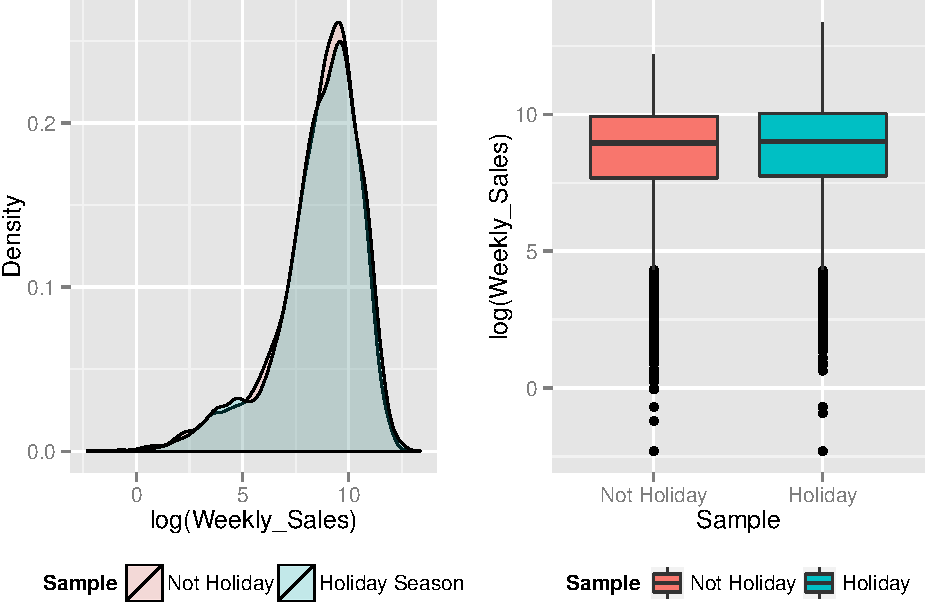
\includegraphics[width=400px]{PredictingWeeklySalesAtWalmart_files/figure-latex/visualizingTheSamplesCollected2-1}

\begin{Shaded}
\begin{Highlighting}[]
\NormalTok{## removing plots from memory}
\KeywordTok{rm}\NormalTok{( xVar , colorVar , sampleDensityDf , plottingDensity , }
    \NormalTok{boxPlotDensity, Hyp_Holiday , Hyp_NotHoliday)}
\end{Highlighting}
\end{Shaded}

\subsubsection{4.2.4 Calculating the Test
Statistic}\label{calculating-the-test-statistic-1}

\begin{Shaded}
\begin{Highlighting}[]
\NormalTok{## Calculating the Difference}
\NormalTok{Diff_Log_Weekly_Sales =}\StringTok{ }\NormalTok{Holiday_Sample -}\StringTok{ }\NormalTok{NotHoliday_Sample}
\NormalTok{## Printing Top 5 values of diff}
\KeywordTok{head}\NormalTok{(Diff_Log_Weekly_Sales)}
\end{Highlighting}
\end{Shaded}

\begin{verbatim}
## [1] -7.3905286 -0.1547533  5.9563873 -5.3583991  4.3064543  2.9671864
\end{verbatim}

\begin{Shaded}
\begin{Highlighting}[]
\NormalTok{## Calculating the Test Statistic}
\NormalTok{xBar <-}\StringTok{ }\KeywordTok{mean}\NormalTok{(Diff_Log_Weekly_Sales)}
\NormalTok{xBar}
\end{Highlighting}
\end{Shaded}

\begin{verbatim}
## [1] 0.1004113
\end{verbatim}

\begin{Shaded}
\begin{Highlighting}[]
\NormalTok{## Calculating the Test Statistic}
\NormalTok{zScore <-}\StringTok{ }\NormalTok{xBar /}\StringTok{ }\KeywordTok{standardError}\NormalTok{(Diff_Log_Weekly_Sales)}
\NormalTok{zScore}
\end{Highlighting}
\end{Shaded}

\begin{verbatim}
## [1] 2.519857
\end{verbatim}

\begin{Shaded}
\begin{Highlighting}[]
\NormalTok{## Calculating p-value}
\NormalTok{## 1-pnorm() because we are doing a one-sided test - greater than}
\NormalTok{pValue <-}\StringTok{ }\DecValTok{1}\NormalTok{-}\KeywordTok{pnorm}\NormalTok{( zScore ) }
\NormalTok{pValue}
\end{Highlighting}
\end{Shaded}

\begin{verbatim}
## [1] 0.005870118
\end{verbatim}

\begin{Shaded}
\begin{Highlighting}[]
\NormalTok{## removing variables not needed anymore}
\KeywordTok{rm}\NormalTok{( pValue , zScore , xBar , Diff_Log_Weekly_Sales , Holiday_Sample , NotHoliday_Sample , ndiff )}
\end{Highlighting}
\end{Shaded}

\subsubsection{4.2.5 Decision: Null Hypothesis (H\textsubscript{0}) is
Rejected}\label{decision-null-hypothesis-h0-is-rejected}

The \textbf{Null Hypothesis (H\textsubscript{0})} is rejected because
the pValue is much smaller than the significance value of 0.05.

This imples that the Alternate Hypothesis (H\textsubscript{A}) is NOT
rejected. Holiday seasons do cause a spike in sales.

\subsubsection{4.2.6 Real World
Application}\label{real-world-application-1}

This confirms the what we visually depicted in Section 3.3.3 regarding
sales spiking up during Christmas and Thanksgiving.

\pagebreak

\subsection{4.3 Do Bigger Stores contribute to Higher Sales
Figures?}\label{do-bigger-stores-contribute-to-higher-sales-figures}

\pagebreak
\# 5. Stage 3: Linear Regression: Predicting Weekly\_Sales

\pagebreak
\# Diagnostic ------- REMOVE LATER

\begin{Shaded}
\begin{Highlighting}[]
\KeywordTok{nrow}\NormalTok{(train)}
\end{Highlighting}
\end{Shaded}

\begin{verbatim}
## [1] 420212
\end{verbatim}

\begin{Shaded}
\begin{Highlighting}[]
\KeywordTok{nrow}\NormalTok{(trainStoresFeaturesMerge)}
\end{Highlighting}
\end{Shaded}

\begin{verbatim}
## [1] 420212
\end{verbatim}

\begin{Shaded}
\begin{Highlighting}[]
\KeywordTok{ls}\NormalTok{()}
\end{Highlighting}
\end{Shaded}

\begin{verbatim}
## [1] "features"                 "lagpad"                  
## [3] "standardError"            "stores"                  
## [5] "test"                     "testStoresFeaturesMerge" 
## [7] "train"                    "trainStoresFeaturesMerge"
## [9] "weekNumber"
\end{verbatim}

\end{document}
